\documentclass[conference]{IEEEtran}
\IEEEoverridecommandlockouts
% The preceding line is only needed to identify funding in the first footnote. If that is unneeded, please comment it out.
\usepackage{cite}
\usepackage{amsmath,amssymb,amsfonts}
\usepackage{algorithmic}
\usepackage{graphicx}
\usepackage{textcomp}
\usepackage{xcolor}
\usepackage{tikz}
\usepackage{multirow}
\usepackage[hidelinks]{hyperref}
\usepackage{multirow}
\usepackage[normalem]{ulem}
\usepackage{makecell}
\useunder{\uline}{\ul}{}
\usetikzlibrary{positioning}

\usepackage[acronym,toc]{glossaries}

\makeglossaries

\def\BibTeX{{\rm B\kern-.05em{\sc i\kern-.025em b}\kern-.08em
    T\kern-.1667em\lower.7ex\hbox{E}\kern-.125emX}}
\begin{document}

\title{Video Super-Resolution using GANs\\
\thanks{978-1-6654-5992-1/22/31.00 ©2023 IEEE}
}

\author{\IEEEauthorblockN{1\textsuperscript{st} Oleh Pomazan}
\IEEEauthorblockA{\textit{Department of Software Engineering} \\
\textit{University of Europe for Applied Sciences}\\
oleh.pomazan@ue-germany.de}
% \and
% \IEEEauthorblockN{2\textsuperscript{nd} Given Name Surname}
% \IEEEauthorblockA{\textit{dept. name of organization (of Aff.)} \\
% \textit{name of organization (of Aff.)}\\
% City, Country \\
% email address or ORCID}
% \and
% \IEEEauthorblockN{3\textsuperscript{rd} Given Name Surname}
% \IEEEauthorblockA{\textit{dept. name of organization (of Aff.)} \\
% \textit{name of organization (of Aff.)}\\
% City, Country \\
% email address or ORCID}
}

% set path where images are stored
\graphicspath{{./img/}}

\maketitle


\begin{abstract}
    Video super-resolution is used to produce high-resolution video frames from the given low-resolution video frames, which can be used in a variety of vision tasks, including video restoration and enhancement, within the entertainment industry and streaming services. \acrfullpl{gan} are widely used for the super-resolution problems and SRGAN \cite{srgan_2016} is the most popular GAN model for \acrfull{sisr}. The SRGAN model uses a complex loss function consisting of pixel-wise \acrfull{mse}, perception, adversarial and total-variation parts. The effects of different components of the loss function on the SRGAN performance were studied by many authors \cite{esrgan_2018,srgan_2016,weighted_srgan_2021} but the role of total-variation loss is not well studied in the context of \acrshort{sisr}.

    In this thesis we study the effect of \acrfull{tv} loss on the performance of SRGAN model in the context of applying \acrlong{sisr} for video frames. The optimal range of the \acrshort{tv} loss weights was found to be between $10^{-8}$ and $10^{-6}$. Larger values of the \acrshort{tv} loss weight cause significant degradation of performance metrics and visible smoothing of the super-resolved frames.

    While the SRGAN model produces high-quality super-resolved images using a single low-resolution frame, it does not utilize additional information from the previous and next frames of the video. Therefore, we investigate the SRGAN model in terms of temporal consistency between the consecutive frames.

\end{abstract}

\begin{IEEEkeywords}
GANs, SRGAN, video super-resolution, total-variation loss
\end{IEEEkeywords}
\begin{tikzpicture}[overlay,remember picture]
\path(current page.north) node(anchor){};
\node[below=of anchor]{IEEE journal paper format};
\end{tikzpicture}

\section{Introduction}
Image \acrfull{sr}is a process of recovering \acrfull{hr} images from \acrfull{lr} images. It is an important category of image processing methods utilized in computer vision, where the goal is to generate one or more \acrshort{hr} images from one or more \acrshort{lr} images. The objective of the SR algorithm is to generate finer details in an image compared to the sampling grid of the imaging device by increasing the pixel density per unit area. \acrshort{sr} is an ill-posed inverse problem, as several HR images can be valid for any given LR image due to many aspects like brightness and coloring. An \acrshort{lr} image, possibly with noise, distortions, and artifacts, is used to restore a \acrshort{hr} image \cite{Hitchhiker_guide_super_res_2023, sr_ill_posed_2021}.

SR finds applications across diverse fields, including satellite imaging and remote sensing, where multiple images of a single area are accessible, in security and surveillance where the need arises to magnify a specific point of interest in a scene (like zooming in on a criminal's face or license plate numbers), in computer vision to enhance pattern recognition performance, and in other domains such as facial image analysis, text image analysis, biometric identification, fingerprint image enhancement, and more \cite{sr_technical_overview_2003}.

\begin{figure}[t]
	\centering
	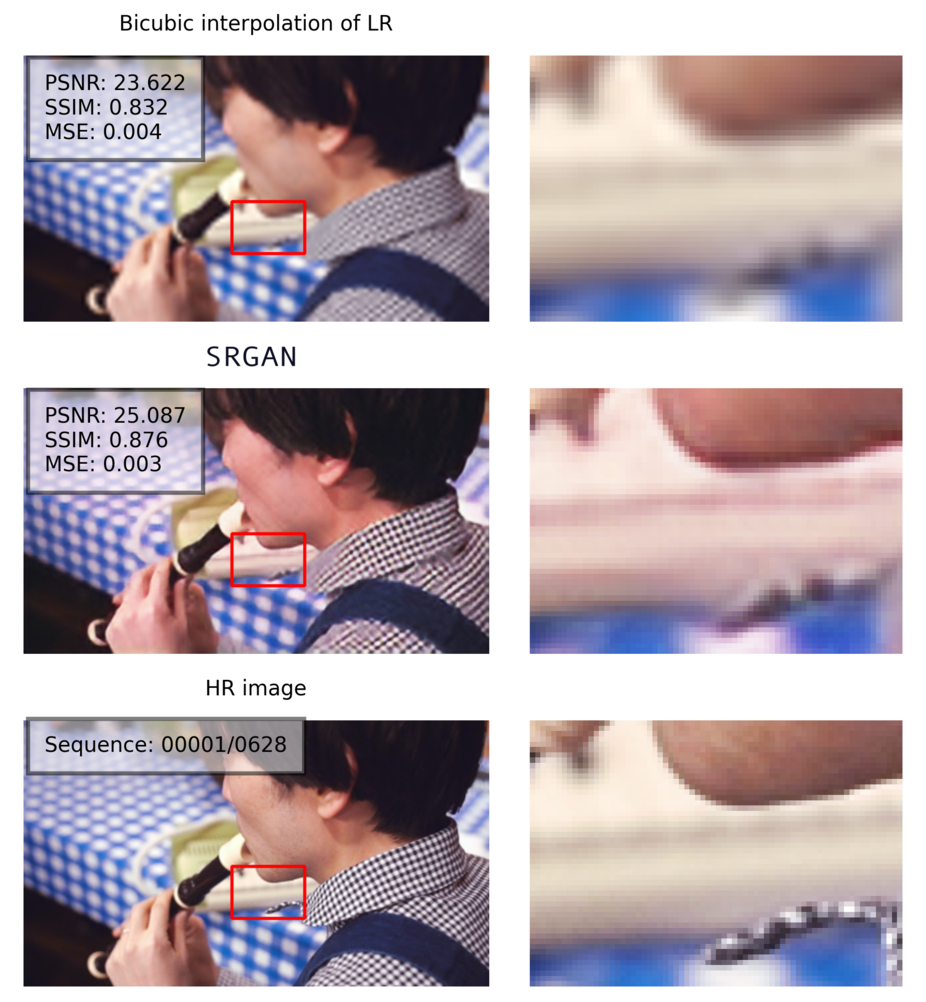
\includegraphics[scale=1.5]{results/crop_00001_0628}
	\caption{Example of the super-resolved frame generated using the SRGAN model (sequence 00001/0628 from Vimeo90K dataset)}
	\label{fig:example_sr_conclusion}
\end{figure}

Video plays an important role in our daily lives, making the enhancement of low-resolution videos through \acrshort{sr} techniques a crucial endeavor. Video super-resolution originates from image super-resolution and has the objective of enhancing the quality of high-resolution videos by reconstructing them from several low-resolution frames. Nevertheless, it is crucial to note that video super-resolution differs notably from image super-resolution since it typically utilizes inter-frame data to achieve its results.

The progress in computing power and deep learning approaches has sparked a multitude of advancements in video-related problems, including frames interpolation, artifact removal, denoising, deblurring, and super-resolution. In this thesis, we focus on \acrshort{vsr} problem applying \acrshort{gan} based approach that is a rapidly developing field.

Over the past few years, there has been a consistent increase in the resolution of consumer devices, including monitors, displays, virtual reality headsets, and other similar technologies. Content that was created in the past may not appear optimal on high-resolution screens for the users. The possibility of real-time \acrshort{vsr} techniques could have significant implications for the entertainment industry, particularly in the context of streaming services. As the demand for streaming platforms continues to soar, applying post-processing VSR approaches on the client side can be feasible, thereby reducing the requirement for large-scale data transfers \cite{video_super_resolution_survey_2020}.

In this work, we investigate existing \acrshort{vsr} approaches based on \acrshortpl{gan} and selected the SRGAN \cite{srgan_2016} model for the research. We study whether \acrlong{sisr} methods based on \acrshortpl{gan} can be applied to \acrlong{vsr} problem and if it can achieve super-resolution performance comparable to \acrshort{vsr} models. We trained several SRGAN models with different parameters on Vimeo90K dataset, see an example of the super-resolved video frame in Fig. \ref{fig:example_sr_conclusion}.

First, we study if the SRGAN model can be used to the \acrshort{vsr} problem and to what temporal inconsistencies and artifacts it can lead. Second, the loss function components are analyzed with emphasis on the total-variation loss. At last, we study the effect of different patch size values on the model's training and performance.

% Three paragraphs defining your field, importance of your topic and why it is significant to work on it today.

% One paragraph defining the work that has been done in this field, with a table summarizing the work that has been done in literature.

% One paragraph defining what has not been done (Gap analysis).

% One paragraph on what you are doing in this work (one main and at least two smaller research questions) and your contribution/novelty of your work.

% One paragraph concluding the introduction section with an overall summary of methods, results, and discussion.

\section{Literature Review}

\subsection{Generative Adversarial Networks}

\Acrfullpl{gan} belong to the class of generative models used in unsupervised machine learning. They consist of two networks, namely the generator and the discriminator, engaged in a competitive zero-sum game framework. \Acrshortpl{gan} employ a latent code that encapsulates all aspects of the generated output.

In the \acrshort{gan} framework, we have two models engaged in a competitive scenario akin to game theory. The setup involves a game with defined payoff functions, where each player strives to maximize their respective payoffs. In this game, one of the networks serves as the generator, which is our main focus and is responsible for producing samples (also known as generated or fake samples) with the goal of imitating those originating from the real training distribution (real samples). The other competing model is the discriminator, which examines the samples and determines whether they are real or fake \cite{gans_overview_2018}.

During training, images or other samples are provided to the discriminator. The discriminator is typically a differentiable function, often implemented as a deep neural network, whose parameters can be learned through gradient descent. When the discriminator is presented with samples/images from the training set (real samples), its objective is to output a value close to one, indicating a high probability that the input is real rather than fake \cite{gans_overview_2018}.

The discriminator is also used to evaluate samples generated by the generator (fake samples), and in this case, the objective of the discriminator is to produce an output as close to zero as possible, indicating that the sample is fake. The generator, on the other hand, is a differentiable function, often implemented as a deep neural network, and its parameters can be learned through gradient descent \cite{gans_overview_2018}.

The generator function operates on a sampled latent vector 'z', which serves as initial noise and acts as a source of randomness to aid the generator in producing a diverse range of outputs. The images generated by the generator are then evaluated by the discriminator, and the generator strives to trick the discriminator into outputting a value of one, making it believe that the generated image is real when, in fact, it is not. For more detailed technical information on \acrshortpl{gan}, readers can refer to \cite{gans_overview_2018}.

\subsection{Video Super-Resolution Overview}

Over the past few years, numerous video super-resolution techniques have emerged, dividing mainly into two categories: traditional approaches and deep learning-based approaches. Traditional super-resolution methods are categorized into three groups: interpolation-based, reconstruction-based, and frequency-based approaches.

So far, many \acrshort{vsr} algorithms have been proposed. Different deep learning models have demonstrated their effectiveness in video super-resolution tasks. Video Super-Resolution typically adopts the multi-input-single-output approach, as it involves providing multiple low-resolution frames to the model to predict a single reference frame. The key emphasis in VSR is on capturing the spatial and temporal relationships between frames.

In Liu et al. \cite{video_super_resolution_survey_2020} the existing VSR methods are categorized into two main categories: methods with alignment and methods without alignment, according to whether the video frames are explicitly aligned.

\begin{figure}[t]
    \centering
    % 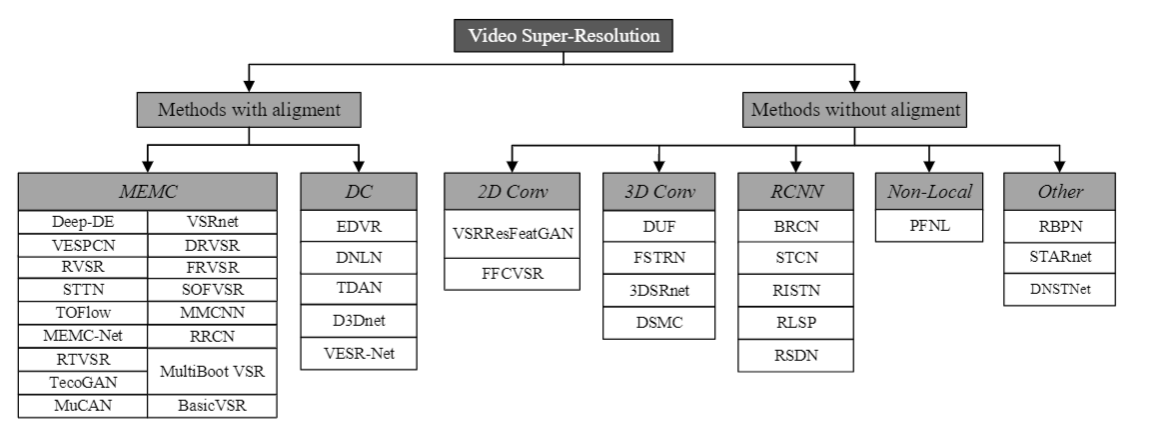
\includegraphics[scale=1]{vsr_methods}
    \centerline{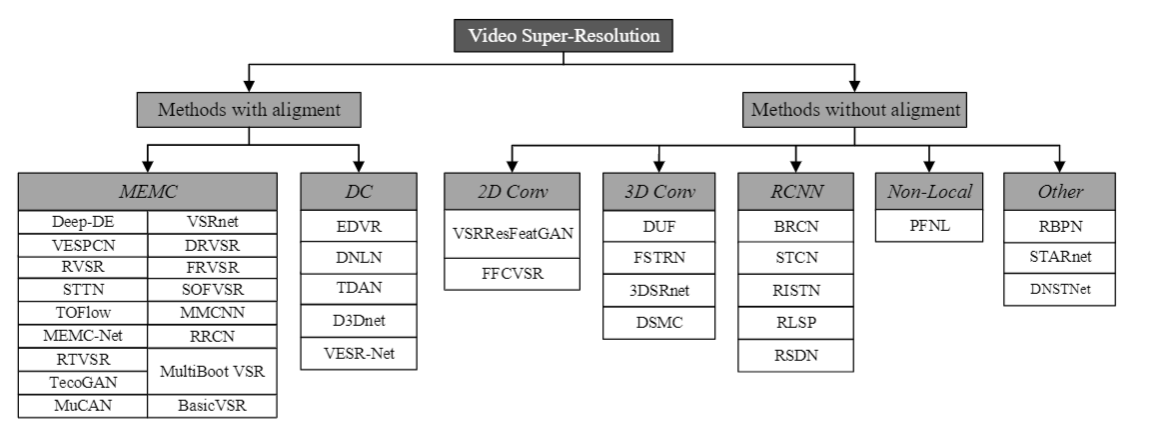
\includegraphics[width=8.9cm]{vsr_methods}}
    \caption{A classification scheme for the current state-of-the-art video super-resolution methods \cite{video_super_resolution_survey_2020}}
    \label{fig:vsr_methods}
\end{figure}

A classification of the current \acrshort{vsr} methods is presented at Fig. \ref{fig:vsr_methods}. There, MEMC stands for Motion Estimation and Compensation, DC is Deformable Convolution, 3D Conv means 3D Convolution and RCNN is Recurrent Convolutional Neural Network \cite{video_super_resolution_survey_2020}.

\subsection{Frame-Reccurent Video Super-Resolution}

Frame recurrent video super-resolution (FRVSR), as proposed by Sajjadi et al. \cite{frvsr_2018}, focuses on using the previously inferred high-resolution (HR) estimate to super-resolve the subsequent frame. This approach aims to achieve temporally consistent results and reduce computational costs. The architecture of FRVSR is presented in Figure \ref{fig:frvsr_arch}.

\begin{figure}[t]
    \centering
    \centerline{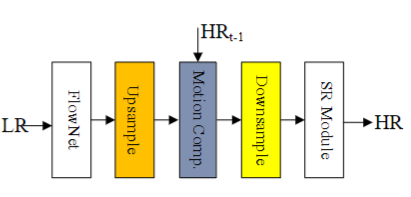
\includegraphics[width=8.9cm]{frvsr_arch}}
    \caption{The network architecture of FRVSR \cite{video_super_resolution_survey_2020}}
    \label{fig:frvsr_arch}
\end{figure}

The detailed implementation involves the use of an optical estimation network to compute the optical flow between the previous frame and the target frame. Subsequently, the low-resolution optical flow is upsampled to match the size of the high-resolution video using bilinear interpolation. The HR variant of the previous frame is then warped using the upsampled LR optical flow, and the warped HR frame is downsampled using space-to-depth transformation to obtain the LR version. Finally, the LR variant of the warped HR frame and the target frame are fed into the subsequent super-resolution network to produce the result for the target frame \cite{video_super_resolution_survey_2020}.

\subsection{TecoGAN}

The Temporally coherent GAN (TecoGAN) by Chu et al. \cite{tecogan_2018} introduces a spatio-temporal discriminator to achieve realistic and coherent video super-resolution. To address recurrent artifacts, they propose a new "Ping-Pong" loss. Similar to GANs, TecoGAN comprises a generator and a discriminator, and its architecture is illustrated in Fig. \ref{fig:tecogan}.

\begin{figure}[b]
    \centering
    \centerline{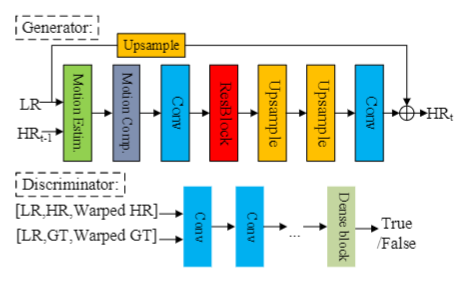
\includegraphics[width=8.9cm]{tecogan}}
    \caption{The network architecture of TecoGAN \cite{video_super_resolution_survey_2020}}
    \label{fig:tecogan}
\end{figure}

\subsection{VSRResFeatGAN}

Rather than employing alignment operations like motion estimation and motion compensation between frames, the input frames are directly fed into a 2D convolutional network for spatial feature extraction, fusion, and super-resolution operations. This approach simplifies the video super-resolution problem by allowing the network to independently learn the correlation information within frames. Representative methods following this approach include VSRResFeatGAN (Lucas et al. \cite{GANs_perc_loss_vsr_2018}) and FFCVSR (Yan et al. \cite{Yan_frame_vsr_2019}).

\subsection{iSeeBetter}

iSeeBetter \cite{iSeeBetter_2020} is a GAN-based spatio-temporal method used for video super-resolution that renders temporally consistent super-resolution videos. iSeeBetter's generator utilizes recurrent back-projection networks to extract spatial and temporal information from both the current and neighboring frames. To enhance the natural appearance of the super-resolved image and eliminate artifacts associated with conventional methods, they incorporate the discriminator from the super-resolution generative adversarial network (SRGAN).

\subsection{Loss function\label{sec:loss_function}}

\begin{figure}[t]
	\centering
    \centerline{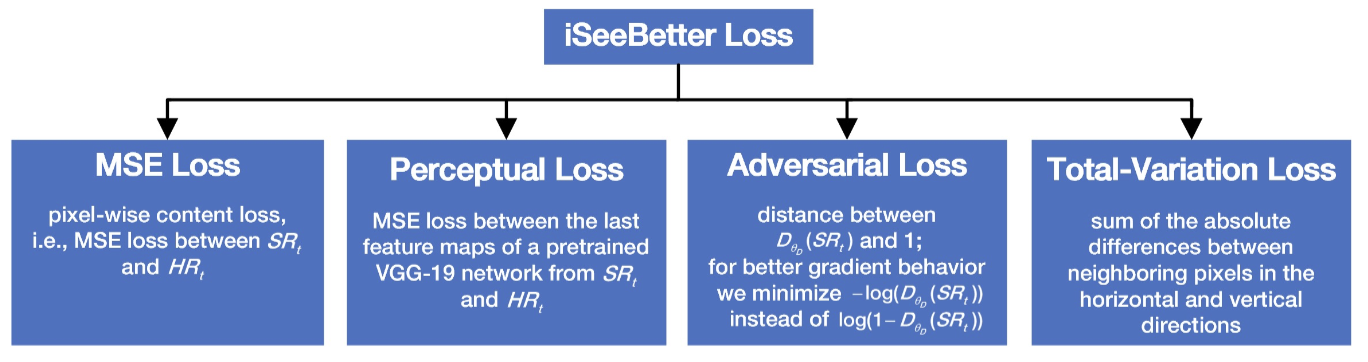
\includegraphics[width=8.9cm]{loss}}
	\caption{The \acrshort{mse}, perceptual, adversarial and \acrshort{tv} loss components \cite{iSeeBetter_2020}.}
	\label{fig:loss}
\end{figure}

The perceptual image quality of the resulting SR image is dependent on the choice of the loss function. To evaluate the quality of an image, MSE is the most commonly used loss function in a wide variety of state-of-the-art SR approaches, which aims to improve the \acrshort{psnr} of an image. Despite optimizing \acrshort{mse} makes better \acrshort{psnr} and \acrshort{ssim} numbers, these metrics do not take into account fine details in the image, potentially misrepresenting the perceptual quality \cite{iSeeBetter_2020}. \acrshort{mse}'s capability to capture intricate texture details by analyzing individual pixel differences in consecutive frames is highly restricted, leading to the potentially excessively smooth video frames \cite{fast_video_super_reso_ann_2012}. Through a sequence of experiments, it was discovered that even when images were deliberately distorted manually, their \acrshort{mse} scores were similar to those of the original, undistorted image \cite{universal_image_quality_index_2002}.

To address this, \cite{iSeeBetter_2020} uses a four-fold (\acrlong{mse}, perceptual, adversarial, and \acrlong{tv}) loss instead of solely relying on pixel-wise \acrshort{mse} loss. Fig. \ref{fig:loss} shows the components of the loss function used in this work.

\subsubsection{Mean-Squared Error Loss}

In this work we use \acrshort{mse} loss (or, alternatively, content loss) for the super-resolved frame $I^{SR}$ against the ground truth $I^{HR}$:

\begin{equation} \label{eq:mse_loss}
	L_{MSE} = \frac{1}{WH} \sum_{x=0}^{W} \sum_{y=0}^{H} ( I^{HR}_{x,y} - G_{\theta_G} (I^{LR})_{x,y} )^2
\end{equation}

where, $G_{\theta_G} (I^{LR})$ is the estimated frame SR, $W$ and $H$ are width and height of the image frames correspondingly \cite{iSeeBetter_2020}.

\subsubsection{Perceptual Loss \label{sec:perceptual_loss}}

Instead of utilizing low-level measures that focus on pixel-wise errors, perceptual loss relies on features extracted from the activation layers of the pre-trained VGG network in the reference paper \cite{vgg_very_deep_cnn_2014}. Perceptual loss, which was introduced in \cite{sr_with_deep_conv_sufficient_stats_2015, texture_synth_cnn_2015}, focuses on perceptual similarity instead of similarity in pixel space.

Here perceptual loss is defined the Euclidean distance between the feature representations of the estimated SR image $G_{\theta_G} (I^{LR})$ and the ground truth image $I^{HR}$:

\begin{gather*} %\label{eq:perceptual_loss}
	L_{perceptual} = \frac{1}{W_{i,j} H_{i,j}} \sum_{x=0}^{W_{i,j}} \sum_{y=0}^{H_{i,j}} ( VGG_{i,j} (I^{HR}_{x,y}) \\- VGG_{i,j} (G_{\theta_G} (I^{LR})_{x,y}) )^2
\end{gather*}

where, $VGG_{i,j}$ is the feature map which is the result of the $j^{th}$ convolution after activation before the maxpooling layer in the VGG network, $W_{i,j}$ and $H_{i,j}$  are the widths and heights of the corresponding feature maps in VGG model \cite{iSeeBetter_2020}.

\subsubsection{Adversarial Loss\label{sec:adversarial_loss}}

Adversarial loss is defined as:

\begin{equation} \label{eq:adversarial_loss}
	L_{adversarial} = -\log ( D_{\theta_D}( G_{\theta_G} (I^{LR}) ) )
\end{equation}

where $D_{\theta_D}$ is the output of the discriminator which is the probability that the reconstructed image $G_{\theta_G} (I^{LR}$ is a real HR image. It was shown in \cite{goodfellow2014generative} that it is better for the gradient behavior to minimize $-\log ( D_{\theta_D}( G_{\theta_G} (I^{LR}) ) )$ instead of $\log (1 - D_{\theta_D}( G_{\theta_G} (I^{LR}) ) )$

\subsubsection{Total-Variation Loss\label{sec:total_variation_loss}}

\acrshort{tv} loss was proposed in \cite{image_upsampling_total_variation_regularization_2005} as a loss function for super-resolution problems. It is defined as the sum of the absolute differences between neighboring pixels in the horizontal and vertical directions. By incorporating TV loss into our overall loss objective, we aim to minimize noise in the input, leading to a denoised output super-resolution image that promotes spatial smoothness.

\acrshort{tv} loss is defined as in \cite{deep_learning_image_sr_2020}:

\begin{gather*} \label{eq:tv_loss}
	L_{TV} = \frac{1}{WH} \sum_{x=0}^{W} \sum_{y=0}^{H}  ((G_{\theta_G} (I^{LR})_{i, j+1} - G_{\theta_G} (I^{LR})_{i, j})^2 + \\(G_{\theta_G} (I^{LR})_{i+1, j} - G_{\theta_G} (I^{LR})_{i, j})^2 )^{\frac{1}{2}}
\end{gather*}

\subsubsection{Loss formulation}

The overall loss objective for each frame is defined as a combination of the MSE, adversarial, perceptual, and TV loss components, with appropriate weights assigned to each component:

\begin{equation} \label{eq:total_Gloss}
	\begin{split}
		L_{G_{\theta_G}} &= \alpha \times L_{MSE}(I^{SR}, I^{HR}) + \\
		& \beta \times L_{perceptual} (I^{SR}, I^{HR}) + \\
		& \gamma \times L_{adversarial}  + \\
		& \delta \times L_{TV} (I^{SR}, I^{HR})
	\end{split}
\end{equation}

where $\alpha, \beta, \gamma, \delta$ are weights.

\subsection{TV loss weight}

\Acrfull{tv} denoising technique is known in image processing \cite{nonlinear_total_variation_noise_removal_1992}. The \acrlong{tv} based loss component was introduced in the original SRGAN paper \cite{srgan_2016} for training of SRResNet-VGG22 model. The \acrshort{tv} loss weight was set to $2 \times 10^{-8}$. The same value of \acrshort{tv} loss $\delta=2 \times 10^{-8}$ is used in \cite{iSeeBetter_2020} and \cite{iSeeBetter_milestone}.

The effect of \acrshort{tv} loss on the performance of the SRGAN model for the face \acrlong{sr} was studied in \cite{SRGAN_with_tv_loss_face_2020} where the \acrshort{tv} loss weight was also set to $2 \times 10^{-8}$ with reference to the SRGAN implementation by Hao Ren \footnote{Github page: https://github.com/leftthomas/SRGAN}.

\Acrshort{tv} loss was used in the research related to the style transfer and \acrlong{sr} \cite{Perceptual_Losses_for_Real_Time_Style_Transfer_and_Super_Resolution_2016} where they set \acrlong{tv} regularization "with a strength of between $1 \times 10^{-6}$ and $1 \times 10^{-8}$, chosen via cross-validation per style target" \cite{Perceptual_Losses_for_Real_Time_Style_Transfer_and_Super_Resolution_2016}.

Following an extensive literature review, we encountered a lack of sufficient explanation for the selected \acrshort{tv} loss weight values utilized in the aforementioned research works. Consequently, we aim to conduct an in-depth investigation into this topic to offer more profound insights into the optimal range of \acrshort{tv} loss weight values for the SRGAN model in the context of the \acrshort{vsr} problem. The summarized review of different \acrshort{tv} vaues is shown in Table \ref{tab:tv_loss_summary}.

\begin{table*}[!tb]
\centering
\caption{Literature review table showing the contributions of various authors for quantization of networks.}
\label{tab:tv_loss_summary}
	\begin{tabular}{|l|c|l|}
	\hline
	  \thead{Paper}                                                     & \thead{TV loss\\weight}       & \thead{Reasoning}                                      \\ \hline
    SRGAN paper \cite{srgan_2016}                             & $2 \times 10^{-8}$   & References to \cite{image_upsampling_total_variation_regularization_2005}, \cite{Perceptual_Losses_for_Real_Time_Style_Transfer_and_Super_Resolution_2016} \\ \hline
	  Faces SR paper  \cite{SRGAN_with_tv_loss_face_2020} & $2 \times 10^{-8}$ & \makecell{Reference to implementation\\(based on \cite{srgan_2016})}  \\ \hline
	  Style transfer paper  \cite{Perceptual_Losses_for_Real_Time_Style_Transfer_and_Super_Resolution_2016} & $10^{-6} - 10^{-8}$  & \makecell{"chosen via cross-validation\\per style target"} \\ \hline
	  iSeeBetter paper \cite{iSeeBetter_2020}              & $2 \times 10^{-8}$        & References to \cite{HandsOn_GANs_2019}                \\ \hline
	  iSeeBetter milestone paper \cite{iSeeBetter_milestone} & $2 \times 10^{-8}$        & References to \cite{single_vsr_gan_pseudo_inverse_2019}                \\ \hline
\end{tabular}
\end{table*}


\section{Methodology}
\subsection{Dataset}

To train the model in this thesis, we use a subset of the original test set of Vimeo90K dataset (not downsampled or downgraded by noise, \(\sim \)15GB of video frames) \cite{vimeo90k_2019}. The septuplet dataset consists of 91,701 7-frame sequences with fixed resolution $448 \times 256$, extracted from 39K selected video clips from Vimeo-90K. This dataset is designed to video denoising, deblocking, and super-resolution. Apart from Vimeo90K dataset, we use other datasets, that are known in the \acrlong{sr} research, for the evaluation of the trained models and comparison of our results with other authors.

\begin{table*}[htb]
    \centering
    \caption{Datasets summary.}
    \label{tab:datasets}
	\begin{tabular}{|l|c|c|c|c|}
	\hline
	Dataset  & Amount & \makecell{Average\\resolution} & Format & Keywords  \\ \hline
	Set5     & 5      & $313 \times 336$   & PNG    & baby, bird, butterfly, head, woman \\ \hline
	Set14    & 14     & $492 \times 446$   & PNG    & humans, animals, insects, etc. \\ \hline
	Urban100 & 100    & $984 \times 797$   & PNG    & architecture, city, structure, urban, etc. \\ \hline
	BSD100   & 100    & $435 \times 367$   & PNG    & animal, building, food, etc. \\ \hline
	Vid4     & 171    & $720 \times 480$   & PNG    &  calendar, city, foliage, walk \\ \hline
\end{tabular}
\end{table*}

\subsection{SRGAN model architecture\label{sec:srgan_arhitecture}}

\begin{figure}[!htb]
	\centering
    \centerline{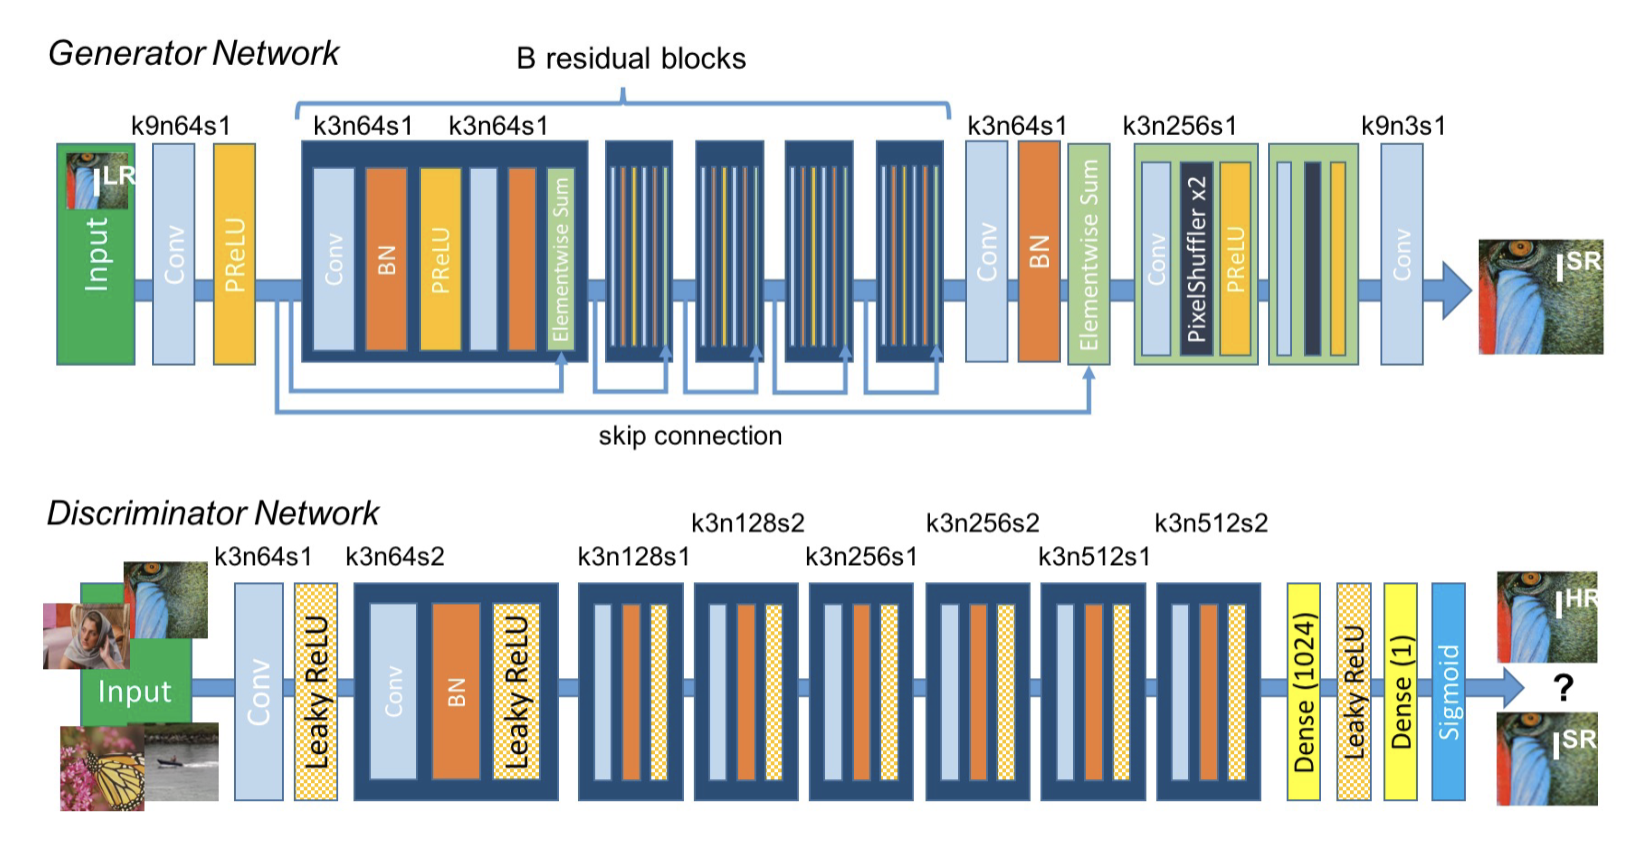
\includegraphics[width=8.9cm]{srgan_model}}
	\caption{Architecture of Generator and Discriminator Network. Here $k$ is the corresponding kernel size, $n$ is a number of feature maps and $s$ is stride indicated for each convolutional layer.}
	\label{fig:srgan_model}
\end{figure}

\acrshortpl{gan} offer a robust framework for generating visually convincing natural images that possess a high level of perceptual quality. The \acrshort{gan} process encourages the generated images to transition towards areas in the solution space that are more likely to contain photo-realistic images. As a result, the generated images become closer to the manifold of natural images, capturing their characteristics and visual realism \cite{goodfellow2014generative}.

We define a discriminator network $D_{\theta_D}$ optimized together with $G_{\theta_G}$ to solve the adversarial min-max problem:

\begin{gather*} \label{eq:adversarial_min_max}
	\min_{\theta_G} \max_{\theta_D} \mathbb{E}_{I^{HR} \sim p_{train} (I^{HR}) }  [ \log D_{\theta_D}(I^{HR})  ] + \\
	\mathbb{E}_{I^{LR} \sim p_G (I^{LR})} [ \log (1 - D_{\theta_D} ( G_{\theta_G} (I_{LR}) )) ]
\end{gather*}

The main concept behind this formulation is to enable the training of a generative model $G$. The objective is to deceive a differentiable discriminator $D$, which is specifically trained to differentiate between super-resolved images and real images. By adopting this approach, the generator network can acquire the ability to generate solutions that closely resemble real images, making them challenging for the discriminator to classify accurately. This strategy promotes the generation of visually superior solutions that align with the characteristics of natural images. In contrast, conventional super-resolution solutions achieved by minimizing pixel-wise error measurements like \acrshort{mse} do not prioritize perceptual quality.

The architecture of the generator network is shown in Fig. \ref{fig:srgan_model}. It consists of $B$ residual blocks with the same layout of two convolutional layers with $3 \times 3$ kernels and 64 feature maps, batch-normalization layers and ParametricReLU \cite{delve_deep_into_rectifiers_2015} as the activation function. The resolution of the input image is increased by two trained sub-pixel convolution layers \cite{sub_pixel_cnn_2016}.

The discriminator network is trained to distinguish between the real HR images from generated SR images. The discriminator architecture is shown in Fig. \ref{fig:srgan_model}. The discriminator model is trained to solve the optimization problem in Equation \ref{eq:adversarial_min_max}. It contains eight convolutional layers with an increasing number of $3 \times 3$ filter kernels, increasing by a factor of 2 from 64 to 512 kernels as in the VGG network \cite{vgg_very_deep_cnn_2014}. Strided convolutions are employed to decrease the image resolution each time the number of features is doubled. After the resulting 512 feature maps there are two dense layers and a final sigmoid activation function to produce a probability for sample classification \cite{srgan_2016}.

\subsection{Detailed Methodology}

We implemented the SRGAN model using PyTorch framework based on the code by Hao Ren \footnote{GitHub page: https://github.com/leftthomas/SRGAN}. Image quality metrics such as \acrshort{psnr}, \acrshort{ssim} and \acrshort{mse} are calculated using TorchMetrics library. We implemented a custom data loader class for Vimeo90K dataset to simplify the training process.

A \emph{research design} guides the execution of a study by encompassing the organization, planning, design, and implementation of the research process.  In this thesis, \emph{experimental research design} was employed, specifically in the form of numerical experiments conducted on a video frames dataset using the SRGAN model. The purpose of these experiments was to assess the hypothesis's viability through the measurement of specific metrics.

To examine the hypothesis that our proposed model outperforms existing methods and holds value in other applications, we adopt a \emph{deductive research approach}. This approach involves systematically testing the hypothesis to either confirm or refute it. The validation of this hypothesis is conducted through quantitative means, specifically by measuring the \acrshort{psnr} and \acrfull{ssim} metrics.

\subsection{Evaluation Metrics}
Video quality refers to the visual attributes of videos, which can be evaluated using either quantitative metrics or perceptual assessments conducted by human viewers. While human assessments offer initial insights, quantitative metrics are essential for benchmarking results and gaining widespread acceptance within the scientific community. This study primarily concentrates on achieving results based on reconstruction accuracy and perceptual naturalness, thereby considering metrics such as \acrfull{mse}, \acrfull{psnr}, and \acrfull{ssim}. These metrics are classified as full-reference metrics, meaning they require both the target (original) and the reconstructed (super-resolved) output to calculate the image/video quality \cite{deep_learning_image_sr_2020}.

\subsubsection{Mean Squared Error}

One widely-used metric is \acrfull{mse}, which is defined by the Equation \ref{eq:mse_metric}:

\begin{equation} \label{eq:mse_metric}
    MSE = \frac{1}{N} \sum_{i}^{N} (\hat{I}_i - \tilde{I}_i)^2
\end{equation}

where $N$ is the total number of pixels in the frame, $\hat{I}$ is the ground-truth HR image, and $\tilde{I}$ is the super-resolved frame.

\subsubsection{Peak Signal to Noise Ratio}

\Acrfull{psnr} is one of the most popular reconstruction quality measurement of lossy transformation such as image compression. For image
super-resolution, PSNR is defined via the maximum pixel value and the \acrshort{mse} between images. \Acrshort{psnr} of one \acrshort{sr} frame is defined as \cite{video_super_resolution_survey_2020}:

\begin{equation}  \label{eq:psnr_metric}
    PSNR = 10 \log_{10} (\frac{L^2}{MSE})
\end{equation}

where $L$ is the maximum range of the pixel color value (usually 255). In general, a higher value of PSNR means superior quality of the image. Because \acrshort{psnr} relies solely on pixel-level \acrshort{mse}, it focuses solely on pixel differences without considering visual perception. Consequently, it often yields unsatisfactory results in representing the true reconstruction quality in real-world scenarios, where human perception matters more. Nevertheless, as a necessity to compare with existing literature and due to the absence of entirely accurate perceptual metrics, PSNR remains the most commonly used evaluation criterion for \acrshort{sr} models \cite{deep_learning_image_sr_2020}.

\subsubsection{Structural Similarity Index Metric}

The \acrfull{ssim} is defined for measuring the structural similarity between images, based on independent comparisons of luminance, contrast, and structures \cite{ssim_2004}. For an image $I$ with $N$ pixels, the luminance $\mu_I = \frac{1}{N} \sum_{i=1}^{N} I(i)$ and contrast $\sigma_I = (\frac{1}{N-1} \sum_{i=1}^{N} (I(i) - \mu_I)^2)^{\frac{1}{2}}$ are calculated as the mean and standard deviation of the image intensity $I$.

The comparisons of luminance and contrast are denoted as $C_l(I, \hat{I})$ and $C_c(I, \hat{I})$ correspondingly, are defined by:

\begin{equation}  \label{eq:comp_luminosity}
    C_l(I, \hat{I}) = \frac{2 \mu_I \mu_{\hat{I}} + C_1 }{\mu_I^2 + \mu_{\hat{I}}^2 + C_1}
\end{equation}

\begin{equation}  \label{eq:comp_contrast}
    C_c(I, \hat{I}) = \frac{2 \sigma_I \sigma_{\hat{I}} + C_2 }{\sigma_I^2 + \sigma_{\hat{I}}^2 + C_1}
\end{equation}

where $C_l = (k_1 L)^2$ and $C_2 = (k_2 L)^2$ are constants preventing instabilities, $k_1 << 1$ and $k_2 << 1$ \cite{deep_learning_image_sr_2020}.

\Acrfull{ssim} is defined as:

\begin{equation}  \label{eq:ssim}
    SSIM(I,\hat{I}) = [C_l(I, \hat{I})]^{\alpha} [C_c(I, \hat{I})]^{\beta} [C_s(I, \hat{I})]^{\gamma}
\end{equation}

where $\alpha$, $\beta$ and $\gamma$ are control parameters for relative importance, $C_s$ is the structure comparison function, defined by:

\begin{equation}  \label{eq:structure_comp_f}
    C_s(I, \hat{I}) = \frac{\sigma_{I\hat{I}}+C_3}{\sigma_I \sigma_{\hat{I}}+C_3}
\end{equation}

where $\sigma_{I, \hat{I}}$ is the covariance between $I$ and $\hat{I}$ and $C_3$ is a constant \cite{deep_learning_image_sr_2020}.

\Acrfull{ssim} is designed as an enhancement over conventional metrics like peak \acrshort{psnr} and \acrshort{mse}. Its purpose is to provide improved performance in assessing the similarity between images.

\section{Results}

\begin{figure}[t]
	\centering
    \centerline{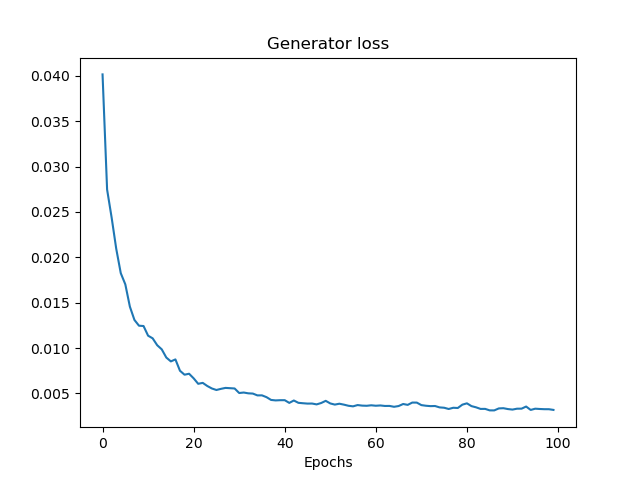
\includegraphics[width=8.9cm]{results/g_loss}}
	\caption{Generator loss during training}
	\label{fig:generator_training_loss}
\end{figure}

\begin{figure}[b]
	\centering
    \centerline{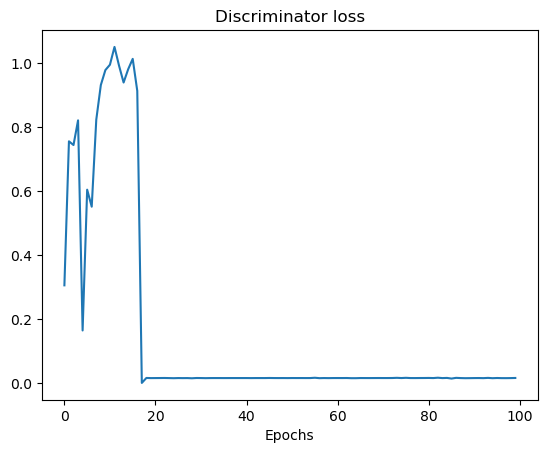
\includegraphics[width=8.9cm]{results/d_loss}}
	\caption{Discriminator loss during training}
	\label{fig:discriminator_training_loss}
\end{figure}

\subsection{Models}

In this work we trained several models with different parameters which define loss function and training hyperparameters such as total-variation weight $\delta$, VGG model for perceptual loss and patch size of HR image during training. The details are shown in the Table \ref{tab:model_parameters}

\begin{figure}[b]
	\centering
    \centerline{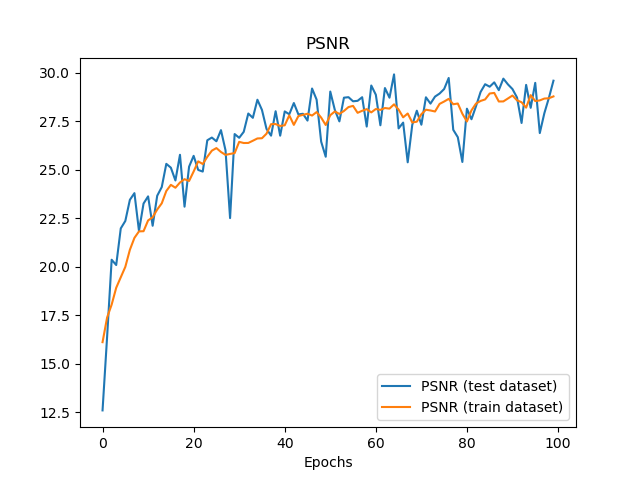
\includegraphics[width=8.9cm]{results/train_psnr}}
	\caption{\acrshort{psnr} metrics during training}
	\label{fig:model_training_metrics}
\end{figure}

All models are trained with upscale factor of $4$. The baseline model uses the same loss weights as in \cite{iSeeBetter_2020}, where \acrshort{mse} loss $\alpha=1$, perceptual loss $\beta=6 \times 10^{-3}$, adversarial loss $\gamma=10^{-3}$ and total-variation loss is $\delta=2 \times 10^{-8}$. All other models were trained using the same \acrshort{mse}, perceptual and adversarial loss weights but with different total-variation loss weights. Their performance is compared to the baseline model further.

\subsection{Model training}

The training process for all models was conducted for 100 epochs. The batch size was set to 196. Adam optimization was employed with a learning rate of 0.001 for both the generator and discriminator networks. The generator network had a total parameter count of 734,092, while the discriminator network had 5,215,425 parameters.

The generator and discriminator losses of $SRGAN_{\delta=0}$ model during training is presented in Fig. \ref{fig:generator_training_loss}, \ref{fig:discriminator_training_loss}. The evolution of performance metrics during training for $SRGAN_{\delta=0}$ model is shown in Fig. \ref{fig:model_training_metrics}.

\subsection{Effect of Total-Variation Loss Weight\label{sec:effect_of_tv_weight}}

We investigated the effect of different total-variation loss values for the performance of the SRGAN model. The performance metrics of the generator network were evaluated with different total-loss weights in the range from 0 to 8. The effect of different values of \acrlong{tv} loss weight on the performance metrics is shown in Fig. \ref{fig:tv_metrics}. Quantitative results are summarized in Table \ref{tab:metrics}

\begin{figure}[htb]
	\centering
    \centerline{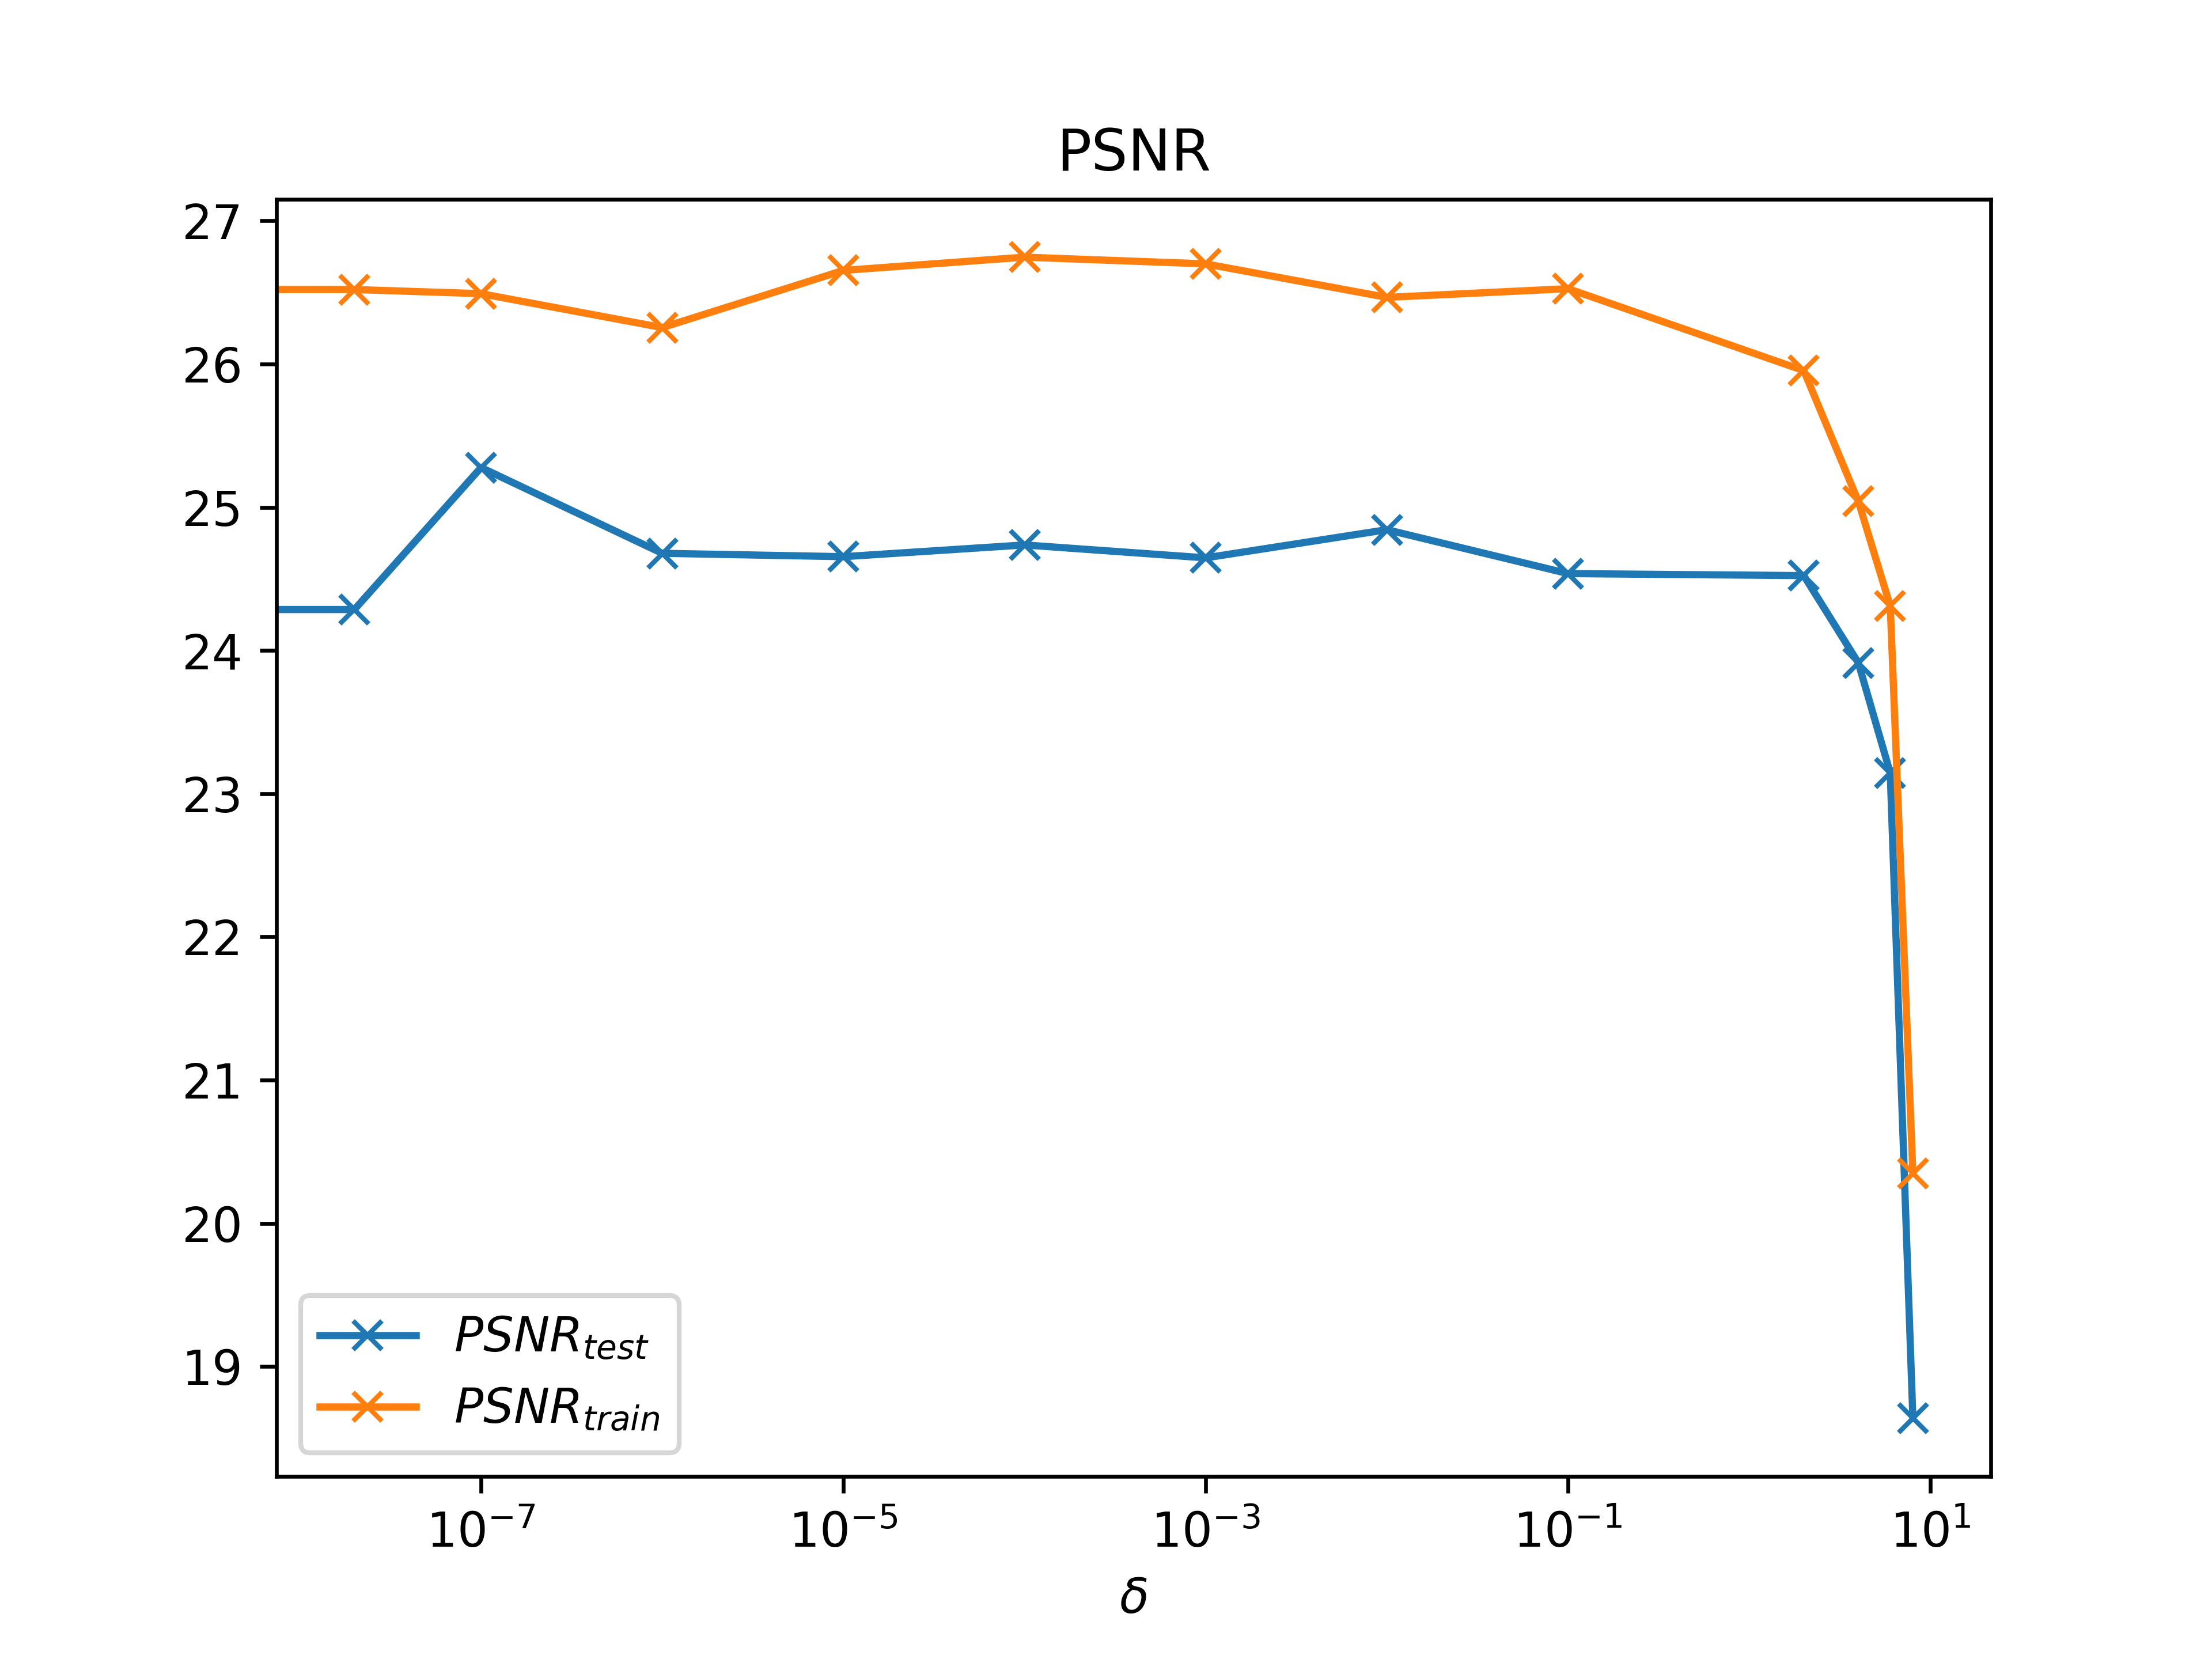
\includegraphics[width=8.9cm]{results/tv_psnr}}
	\caption{\acrshort{psnr} for different values of TV loss weight $\delta$}
	\label{fig:tv_metrics}
\end{figure}

The best performance metrics were demonstrated for the $SRGAN_{\delta=10^{-7}}$ model: $MSE=0.0033$, $PSNR=25.277$ and $SSIM=0.796$.

It was found that models trained with $\delta > 2$ starts to produce increasingly smooth super-resolved images due to the effect of total-variation spatial smoothing \cite{image_upsampling_total_variation_regularization_2005}. For instance, the results obtained using $SRGAN_{\delta=4}$ model are presented in Fig. \ref{fig:tv_1e_7_seq_00001_0629}. This model was trained with \acrshort{tv} loss $\delta=4$. It is visible that the resulting super-resolved images are oversmooth and worse by metrics in comparison to bicubic interpolation baseline images. Model performance metrics are also worse in comparison to the baseline model.

\begin{figure}[htb]
	\centering
    \centerline{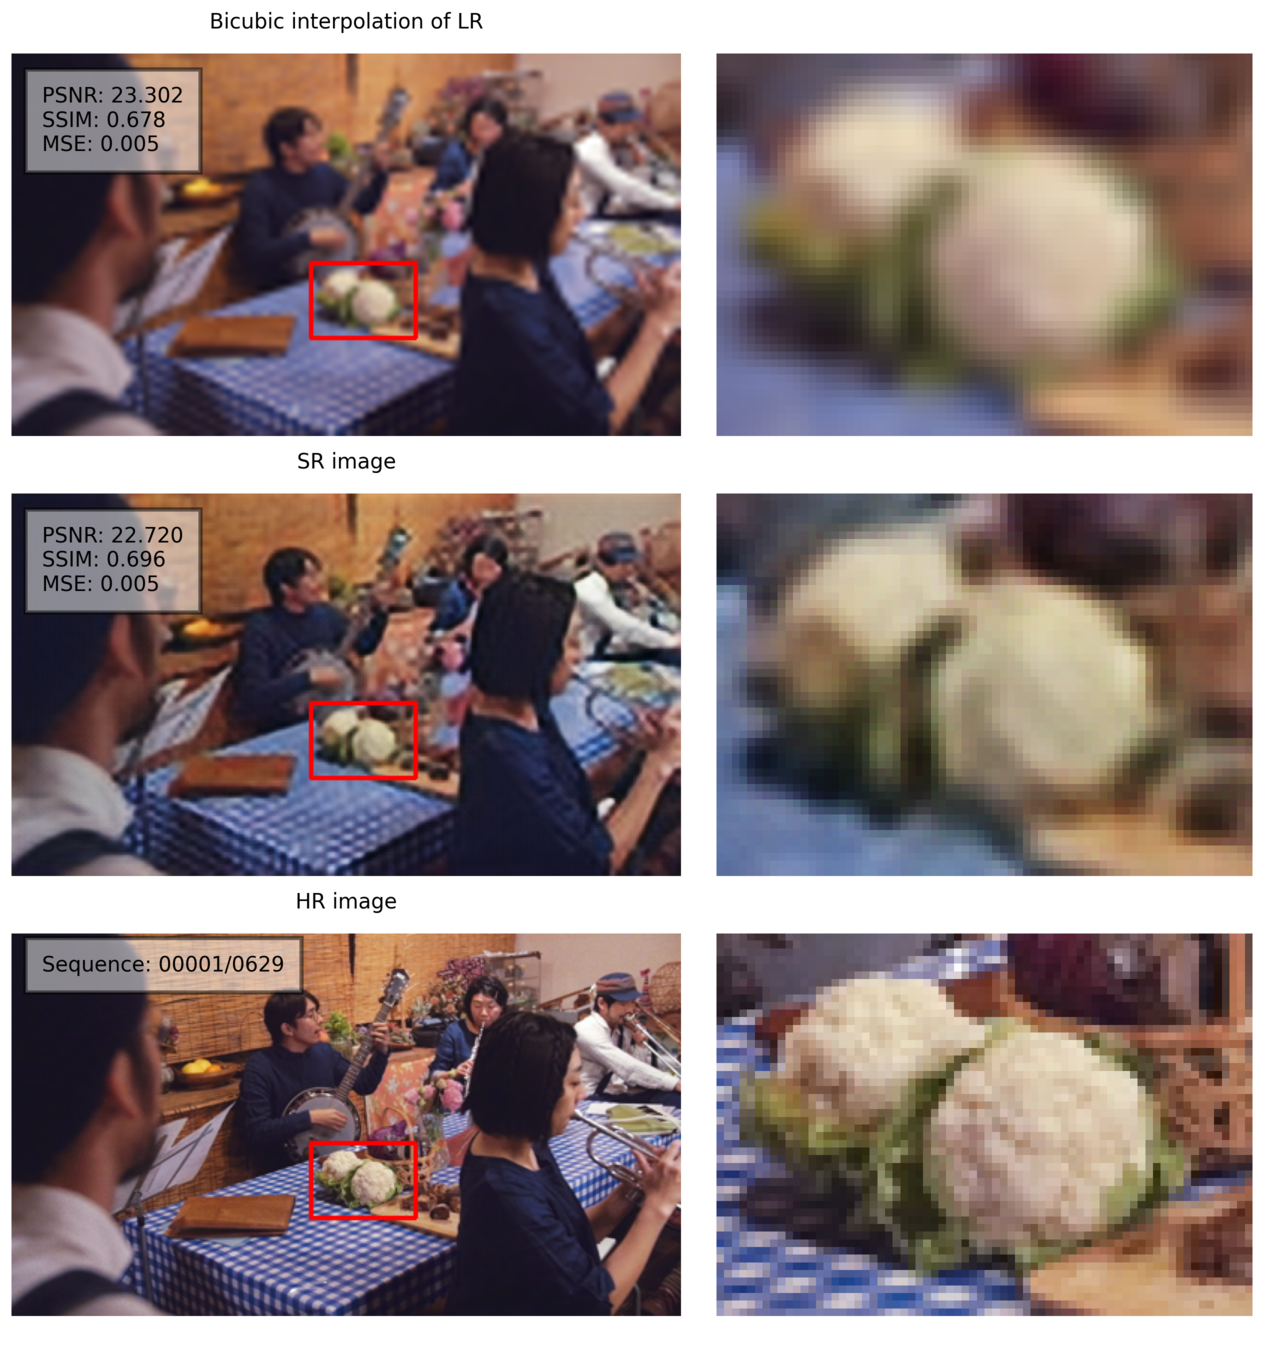
\includegraphics[width=8.9cm]{results/00001_0629}}
	\caption{$SRGAN_{\delta=10^{-7}}$ model for sequence 00001/0629 from the dataset \cite{vimeo90k_2019}}
	\label{fig:tv_1e_7_seq_00001_0629}
\end{figure}

\begin{figure}[htb]
	\centering
    \centerline{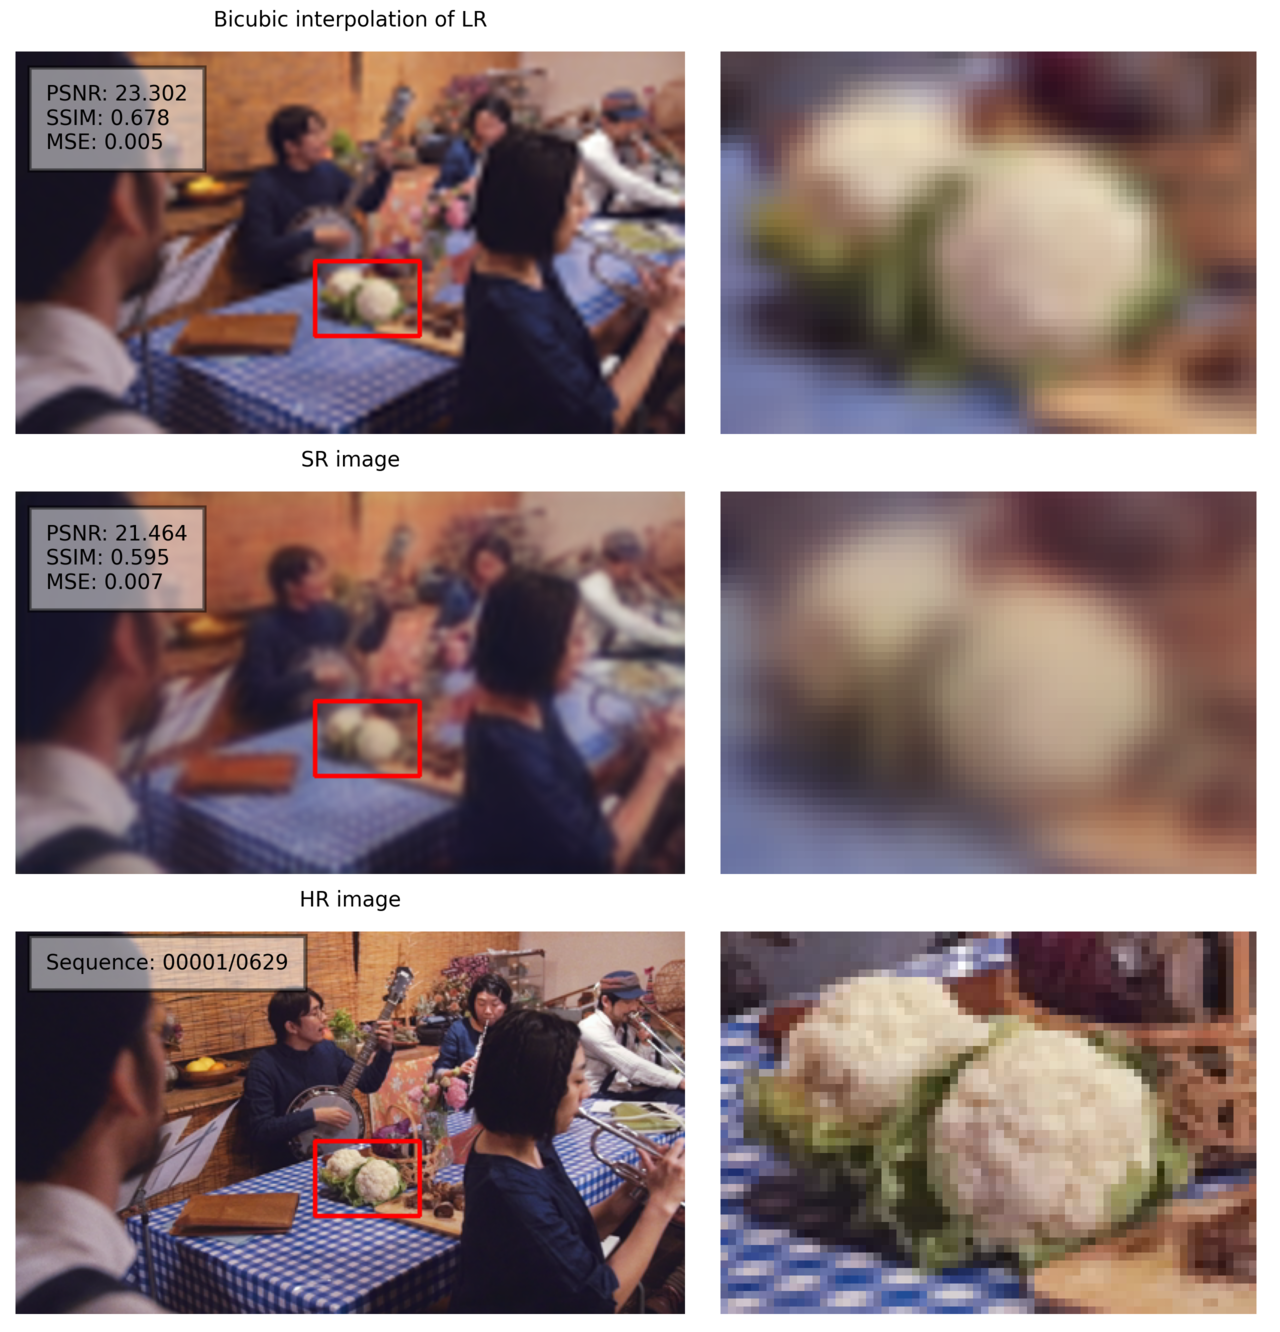
\includegraphics[width=8.9cm]{results/tv_4_00001_0629}}
	\caption{$SRGAN_{\delta=4}$ model for sequence 00001/0629 from the dataset \cite{vimeo90k_2019}}
	\label{fig:tv_4_seq_00001_0629}
\end{figure}

\subsection{Perceptual Loss: VGG16 vs VGG19 \label{sec:vgg_16_vs_19}}

Perceptual loss relies on features extracted from the activation layers of the pre-trained VGG network and it is discussed in \ref{sec:perceptual_loss}.

The baseline model $SRGAN_{baseline}$ was trained using perception loss which is based on VGG16 convolutional neural network \cite{vgg_very_deep_cnn_2014}. It contains 16 hidden layers. We trained $SRGAN_{VGG19}$ model to check how it affects the performance metrics of the model in comparison to baseline model. VGG19 convolutional neural network was used in the original SRGAN model \cite{srgan_2016}. It appears that on the test dataset\newline $SRGAN_{VGG19}$ demonstrates slightly higher \acrshort{ssim} metric but lower \acrshort{psnr} metric (see Table \ref{tab:models_metrics_summary}).

\subsection{Effect of different patch sizes on model training and performance}

During the training we do not use the whole HR images as an input for the generator because it would significantly increase the computational requirements. Instead, we use random patches of $64 \times 64$ size cropped from the original images to speed up the training process.

We trained $SRGAN_{128 \times 128}$ model with baseline parameters and the patch size of $128 \times 128$ pixels.  $SRGAN_{128 \times 128}$ demonstrates significantly better results than the baseline model $SRGAN_{64 \times 64}$ trained with patch size $64 \times 64$. The performance metrics for both models on the test dataset are presented in Tab. \ref{tab:models_metrics_summary}.

\subsection{Evaluation on popular datasets\label{sec:eval_on_datasets}}

The ability of a model to generalize plays a crucial role in assessing how well it can maintain its performance when tested on unfamiliar data that differs from what it was trained on. We trained our model on Vimeo90K dataset (test set for video super-resolution) \cite{vimeo90k_2019} which contains frames of size $448 \times 256$.

We conducted evaluation of the two models trained using the patch sizes of $64 \times 64$ and $128 \times 128$ on the datasets mentioned in \cite{weighted_srgan_2021}: Set5 \cite{set5_2012}, Set14 \cite{Set14_2012}, Urban100 \cite{urban100_2015} and BSD100 \cite{BSD100_2001}. The performance metrics of the trained models are compared to the Weighted SRGAN model (WSRGAN) metrics from \cite{weighted_srgan_2021} with \acrshort{mse} weight of 0.9 and perceptual loss weight of 0.1. The comparison of metrics calculated on the mentioned datasets are summarized in Tab. \ref{tab:models_metrics_summary}.

\subsection{Temporal profiles\label{sec:temporal_profiles}}

The most effective way to assess the consistency of the results over time is through visual examination of the video output. We adopt the approach used by Caballero et al. \cite{Real_Time_Video_Super_Resolution_with_Spatio_Temporal_Networks_and_Motion_Compensation_2016} which employs temporal profiles, as depicted in Fig. \ref{fig:city_temporal_profile}. A temporal profile is created by extracting the same horizontal row of pixels from multiple frames in the video and arranging them vertically to form a new image. Any flickering observed in the video will be evident in the temporal profile as jitter and jagged lines \cite{frvsr_2018}.

There are visible checkboard artifacts on the City temporal profile (Fig. \ref{fig:city_temporal_profile}). It means that some pixels experience intermittent changes in their brightness levels leading to the flickering effect on the video.

% city
\begin{figure}[htb]
	\centering
    \centerline{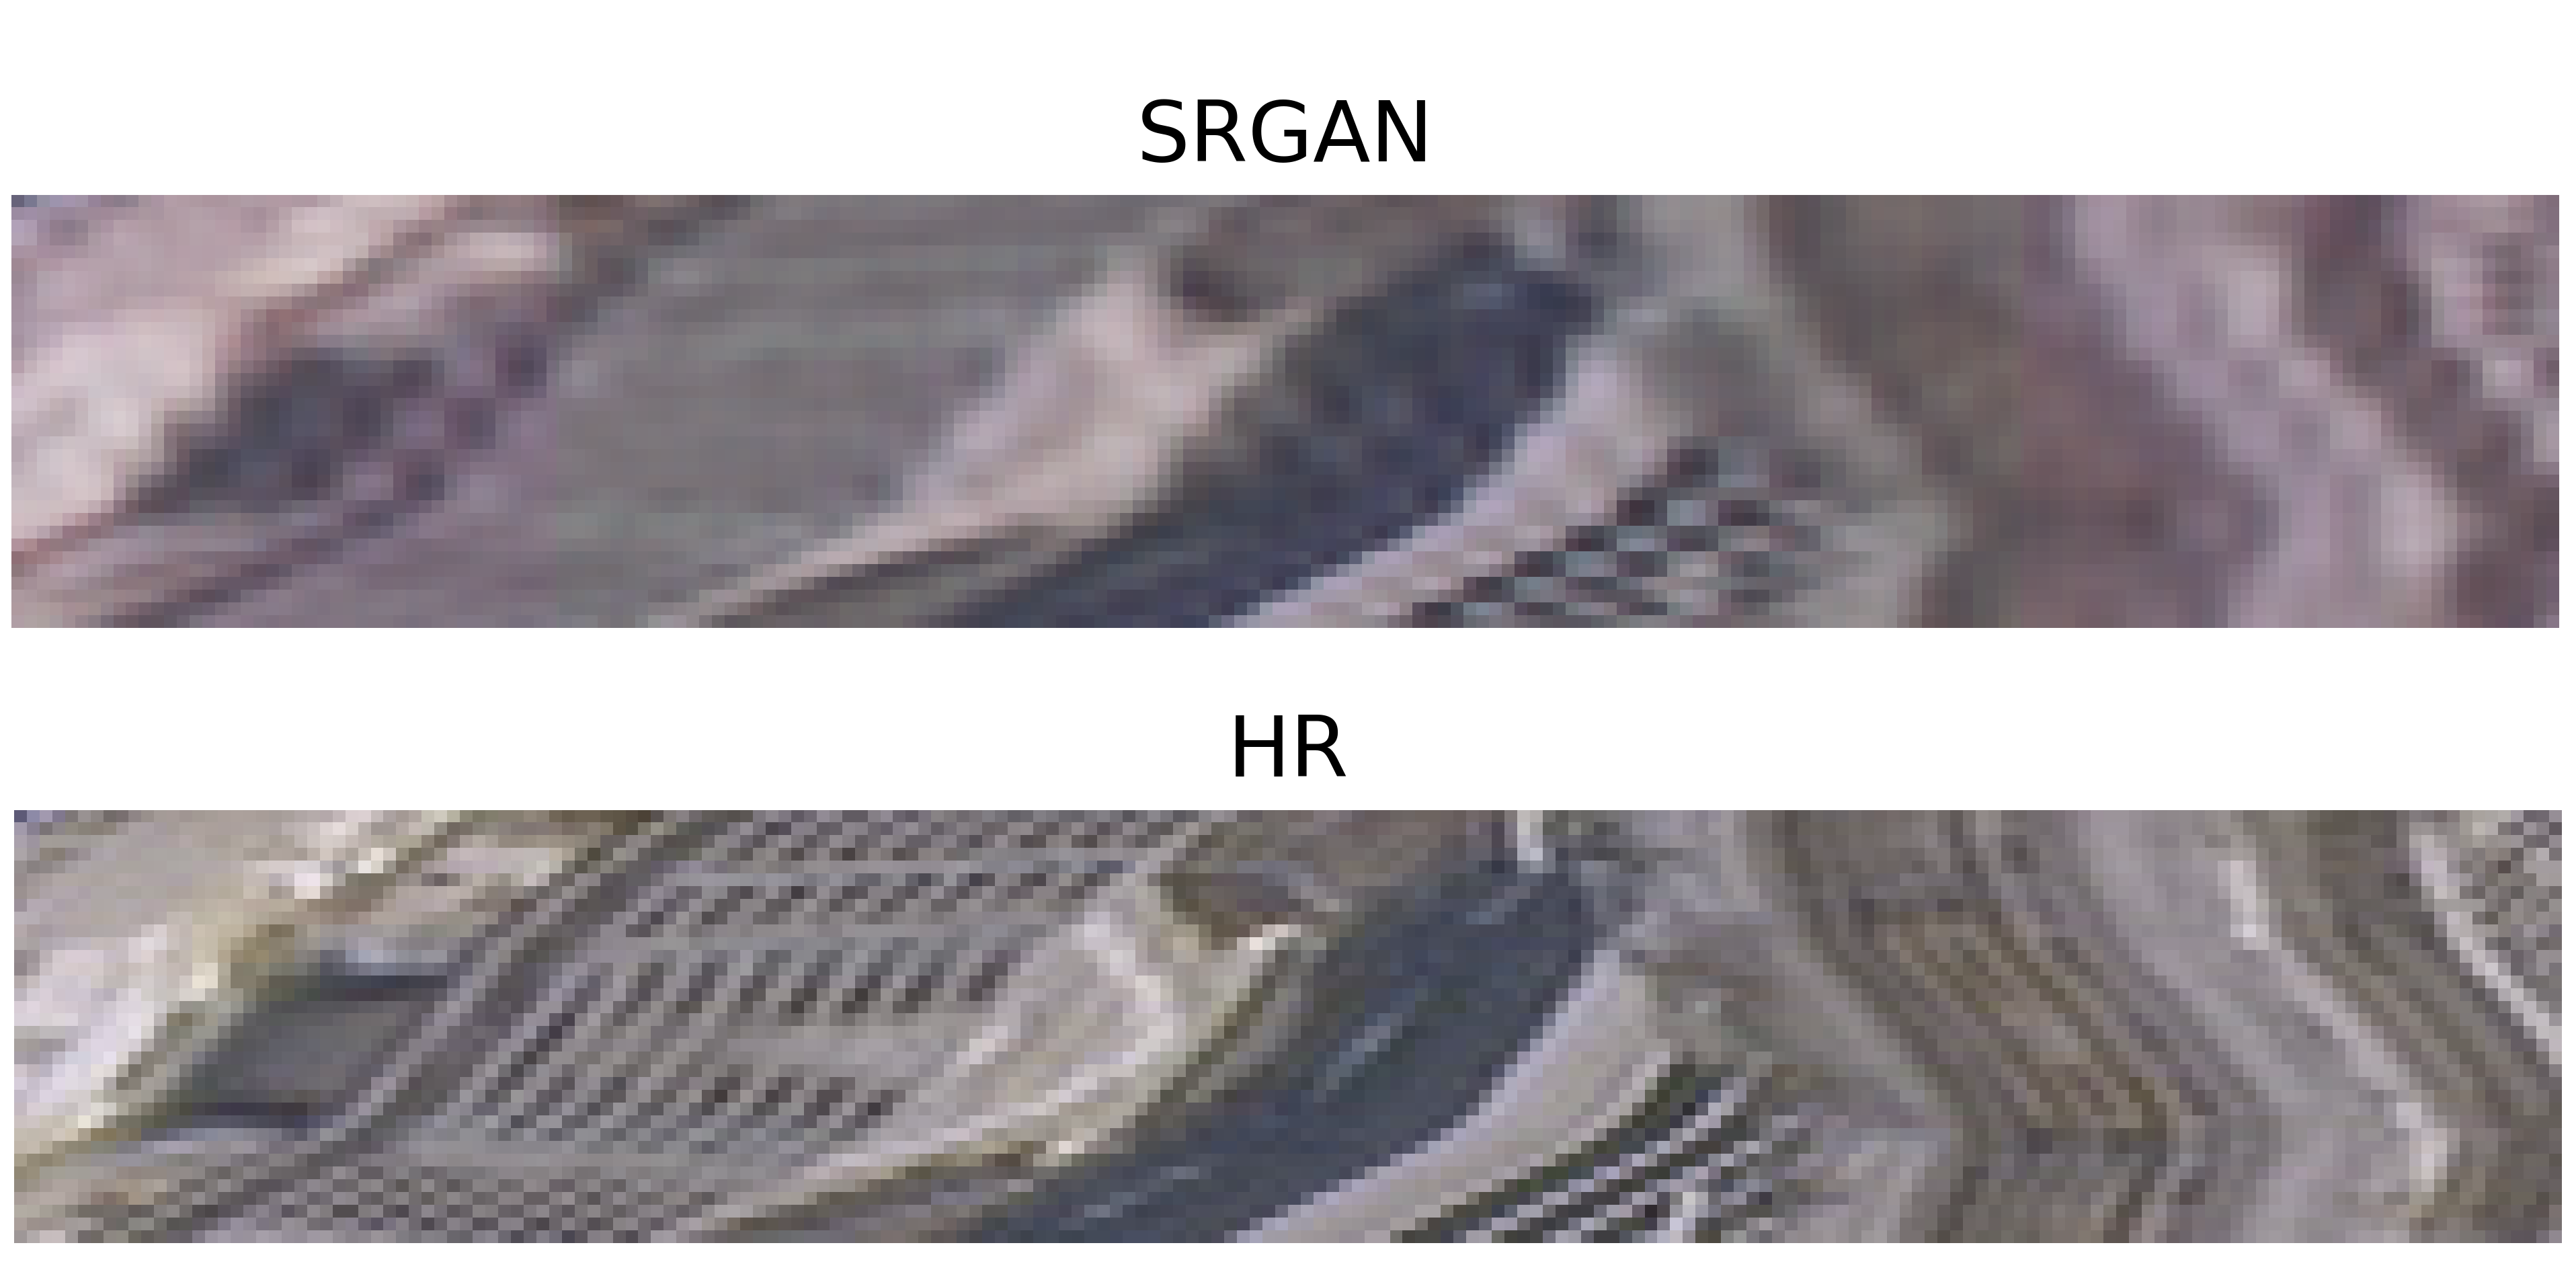
\includegraphics[width=8.9cm]{results/tempo/city_temp_profile}}
	\caption{Temporal profiles for City video sequence from Vid4 dataset.}
	\label{fig:city_temporal_profile}
\end{figure}

\section{Discussion}

\subsection{Effect of Total-Variation Loss}

Since the inclusion of \acrshort{tv} loss as a component of our overall loss objective serves to reduce noise in the input, thereby aiding in the denoising of the output \acrshort{sr} image. As a result, this encourages spatial smoothness in the final \acrshort{sr} image \cite{iSeeBetter_2020}. This is the effect that was expected from the addition of \acrshort{tv} component to the total loss.

In our experiments, we trained 12 SRGAN models with different values of \acrshort{tv} loss weight in order to measure the performance metrics of the trained SRGAN models. The \acrshort{tv} loss weights were in the range between $10^{-8}$ and $8$. The results are presented in Table. \ref{tab:metrics}.

The highest performance metrics were demonstrated for the $SRGAN_{\delta=10^{-7}}$ model:\newline $MSE=0.0033$, $PSNR=25.277$ and $SSIM=0.796$ on the test dataset. The baseline model $SRGAN_{\delta={2 \times 10^{-8}}}$ demonstrated similar performance metrics: $MSE=0.0045$,\newline $PSNR=24.286$ and $SSIM=0.795$. We found that the quality of the \acrshort{sr} images started to deteriorate for $\delta > 2$. It is visible by performance metrics (Fig. \ref{fig:tv_metrics}) and visually (Fig. \ref{fig:tv_4_seq_00001_0629}).

The \acrshort{tv} loss is calculated according to Equation \ref{eq:tv_loss} in Section \ref{sec:total_variation_loss}. In order to understand why the SRGAN model performance degrade when the \acrshort{tv} loss weight is more than 2 we can use the baseline SRGAN model's generator and discriminator trained with $\delta = 2 \times 10^{-8}$ to calculate the total loss and the loss components while varying the \acrshort{tv} loss weight. The generator is required to produce the \acrshort{sr} images and the discriminator calculates the probability that the fake image is the real \acrlong{hr} image. It is used in the calculation of the adversarial loss, see Section \ref{sec:adversarial_loss}.

The calculated components of the generator loss are shown in Fig. \ref{fig:tv_loss_components}. \acrshort{mse}, adversarial and perceptual losses are independent of the \acrshort{tv} value loss, therefore they are represented by horizontal lines on the plot. \Acrshort{tv} loss is almost 0 for $\delta < 10^{-1}$ and does not affect the total loss of the generator until $\delta > 10^{-1}$. After this point, the \acrshort{tv} loss starts to contribute significantly to the total loss and it coincides with the drop in performance metrics of the trained models (see Fig. \ref{fig:model_training_metrics}).

\begin{figure}[htb]
	\centering
    \centerline{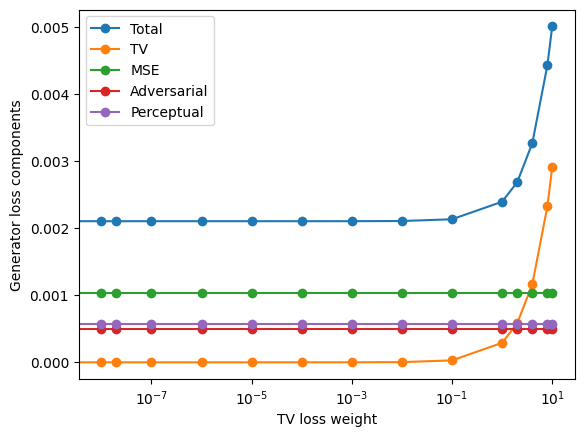
\includegraphics[width=8.9cm]{results/tv_loss_components}}
	\caption{Generator loss components for different values of the TV loss weight}
	\label{fig:tv_loss_components}
\end{figure}

The super-resolved images generated by the SRGAN model, which was trained with a high \acrlong{tv} loss weight, exhibit excessive smoothness and a deficiency in capturing fine texture details (Fig. \ref{fig:tv_smooth_comparison}). This outcome can be attributed to a shift in the training objective, where the components of the total loss that assess image quality (such as \acrshort{mse} and perception losses) are overshadowed by \acrshort{tv} loss contribution to the total loss.

\begin{figure}[htb]
	\centering
    \centerline{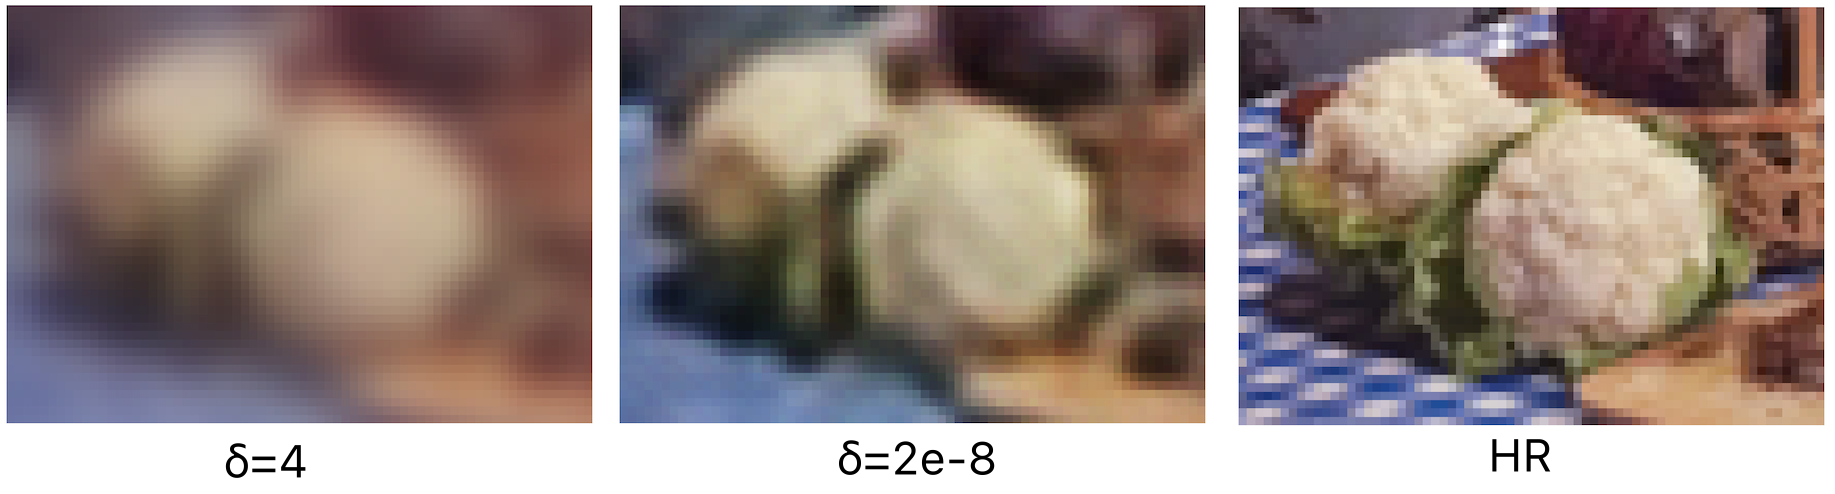
\includegraphics[width=8.9cm]{results/tv_smooth_comparison}}
	\caption{Visual example of oversmoothness of the super-resolved imaged for large values of the TV loss weight.}
	\label{fig:tv_smooth_comparison}
\end{figure}

From the experiments carried out, it can be inferred that while training the SRGAN model, it is advisable to employ a low \acrlong{tv} (TV) loss weight within the range of $10^{-8}$ to $10^{-6}$. If larger values of the \acrshort{tv} loss weight are used, it can lead to an unreasonable smoothness of the super-resolved images, which is undesirable for the \acrlong{sr} (SR) problem, as it results in the loss of crucial texture details on smaller scales. The suggested range aligns with values utilized by other researchers (see Table \ref{tab:tv_loss_summary}).

\subsection{Temporal profiles}

After conducted experiments and analyzed results we can say that it is definitely possible to apply the SRGAN model for \acrshort{vsr} problem in order to generate \acrshort{sr} frames. However, it should be noted, that there are limitations to such approach that are result of the specific distortions and artifacts from temporal inconsistencies between frames.

We research such inconsistencies following the approach from Caballero et al. \cite{Real_Time_Video_Super_Resolution_with_Spatio_Temporal_Networks_and_Motion_Compensation_2016} where the temporal profile is generated by taking the same horizontal row of pixels from a number of frames in the video and stacking them vertically into a new image.

Temporal inconsistencies similar to those mentioned in Mehdi et al. \cite{frvsr_2018} were not observed in our study when analyzing the temporal profiles. The hypothesis is that the quality of the generated \acrshort{sr} frames by the trained SRGAN model on the Vid4 dataset is not enough to reveal finer details of the frames. These \acrshort{sr} frames lack the necessary level of detail, resulting in oversmoothed appearances and a lack of texture details. As a consequence, the discrepancies between consecutive frames are not evident.

\begin{figure}[!htb]
	\centering
    \centerline{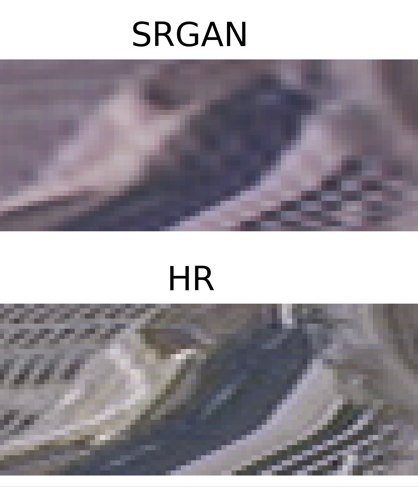
\includegraphics[width=5cm]{results/tempo/checkboard_artifacts}}
	\caption{Checkerboard artifacts in the temporal profiles}
	\label{fig:checkerboard_artifacts}
\end{figure}

Instead, we notice other kinds of artifacts and distortions such as checkerboard artifacts on the City sequence temporal profile from Vid4 (see Fig. \ref{fig:city_temporal_profile} and Fig. \ref{fig:checkerboard_artifacts}). The primary source of checkerboard artifacts in the \acrshort{sr} images stems from two key processes: forward-propagation during upsampling, which involves transposed convolutional layers, and backward-propagation during downsampling, which employs strided convolutional layers \cite{checkerboard_2020}. These specific operations contribute significantly to the emergence of checkerboard artifacts in the generated \acrshort{sr} images.

It should be noted that here we have a similar effect but on the temporal profile instead of the super-resolved image. The precise reason behind the appearance of checkerboard artifacts in the temporal profiles of the super-resolution (\acrshort{sr}) images is an open question. However, this phenomenon results in pixel brightness fluctuations in the video, leading to a flickering effect \cite{frvsr_2018}. The specific cause of these artifacts in the \acrshort{sr} images is still an unresolved aspect that requires further investigation.

\subsection{Effect of Hyperparameters Tweaking}

\subsubsection{Patch size}

In ideal circumstances the model is trained on the whole images available in the dataset. Throughout the training process, the entire high-resolution images are not used as input for the generator. Using the complete images would substantially escalate the computational demands. Instead, to conduct the training, random patches of size $64 \times 64$ are cropped from the original images and used. The objective in this case was to measure how increased patch size influences the performance and training time of the SRGAN model trained with the same number of epochs.

One model with the patch size $128 \times 128$ was trained. We found that training the process of $SRGAN_{128 \times 128}$ model is similar to the training of $SRGAN_{64 \times 64}$, but the requirements for the GPU memory is higher. We had to decrease the batch size from 196 to 32. The  $SRGAN_{128 \times 128}$ model training for 100 epochs took approximately 3 hours, and for $SRGAN_{128 \times 128}$  it took 90 minutes (average value for 12 trained models). The training parameters are summarized in Table \ref{tab:crop_64_vs_128_results}. The \acrshort{mse}, \acrshort{ssim} and \acrshort{psnr} metrics are presented in Table \ref{tab:models_metrics_summary}.

The train time is increased by the factor of 2. It is evident that increased patch size provides significant improvement for visual quality of the super-resolved images and metrics are also higher.

\subsubsection{VGG16 vs VGG19}

Perceptual loss relies on features computed by the activation layers of the pre-trained VGG network (see Section \ref{sec:perceptual_loss}). All trained models use perception loss which is based on VGG16 convolutional neural network with 16 hidden layers \cite{vgg_very_deep_cnn_2014}. In order to estimate how it affects the performance metrics of the model in comparison to baseline model, we trained $SRGAN_{VGG19}$ model with 19 hidden layers from VGG19 network. The VGG19 pre-trained model is provided by PyTorch framework.

The experiment reveals that on the test dataset, $SRGAN_{VGG19}$ exhibits a slightly higher \acrlong{ssim} (SSIM) metric but a lower \acrlong{psnr} (PSNR) metric (refer to Table \ref{tab:models_metrics_summary}). However, visually assessing the difference proves to be subjective. There was no significant difference in the train time between the two models as it took ~90 minutes to train both. Hence, it makes sense to use deeper VGG model to increase the influence of perception loss of the SRGAN model without incurring additional training time penalty.

\section{Conclusion}

This research focuses on applying the SRGAN model to address the \acrlong{vsr} problem by employing it on a per-frame basis for video sequences. Our contributions in the realm of \acrlong{vsr} encompass two key aspects: firstly, we analyzed the impact of \acrlong{tv} loss weight on the SRGAN model's performance when trained on video sequences, and secondly, we investigated the temporal characteristics of the super-resolved frames to identify any temporal inconsistencies.

Through our work, we demonstrated that the SRGAN model can indeed be employed for solving the \acrlong{vsr} problem while also shedding light on its limitations. By generating temporal profiles, we delved into temporal inconsistencies, artifacts, and distortions that restrict the suitability of the \acrlong{sisr} approach for enhancing the resolution of video frames.

\bibliographystyle{IEEEtran}
\bibliography{Bibliography}

\section{Reference material}

\begin{table*}[htb]
	\centering
	\caption{The SRGAN model performance metrics (\acrshort{mse}, \acrshort{psnr} and \acrshort{ssim})}
	\label{tab:metrics}
	\begin{tabular}{|c|c|c|c|}
	\hline
	Total-variation loss weight $\delta$ & $MSE_{test}$ & $PSNR_{test}$ & $SSIM_{test}$  \\ \hline
	$0$                                 & 0.0042       & 24.334        & 0.789          \\ \hline
	$2 \times 10^{-8}$                  & 0.0045       & 24.286        & 0.795          \\ \hline
	$10^{-7}$                           & 0.0033       & 25.277        & 0.796          \\ \hline
	$10^{-6}$                           & 0.0039       & 24.678        & 0.790          \\ \hline
	$10^{-5}$                           & 0.0038       & 24.655        & 0.785          \\ \hline
	$10^{-4}$                           & 0.0038       & 24.737        & 0.791          \\ \hline
	$10^{-3}$                           & 0.0039       & 24.647        & 0.784          \\ \hline
	$10^{-2}$                           & 0.0037       & 24.843        & 0.792          \\ \hline
	$10^{-1}$                           & 0.0038       & 24.537        & 0.789          \\ \hline
	$2$                                 & 0.0041       & 24.522        & 0.782          \\ \hline
	$4$                                 & 0.0046       & 24.913        & 0.755          \\ \hline
	$6$                                 & 0.0055       & 24.145        & 0.724          \\ \hline
	$8$                                 & 0.0161       & 18.638        & 0.673          \\ \hline
\end{tabular}
\end{table*}

\begin{table*}[htb]
	\centering
	\caption{Parameters of the trained models, where $\alpha$, $\beta$, $\gamma$ and $\delta$ are correspondingly \acrshort{mse}, perceptual, adversarial and total-variation loss weights (see Equation \ref{eq:total_Gloss})}
	\label{tab:model_parameters}
	\begin{tabular}{|l|c|c|c|c|c|c|}
	\hline
	Model                    & $\alpha$ & $\beta$            & $\gamma$  & $\delta$           & Patch size       & VGG model      \\ \hline
	$SRGAN_{baseline}$       & 1        & $6 \times 10^{-3}$ & $10^{-3}$ & $2 \times 10^{-8}$ & $64 \times 64$   & VGG16          \\ \hline
	$SRGAN_{\delta=0}$       & 1        & $6 \times 10^{-3}$ & $10^{-3}$ & $0$                & $64 \times 64$   & VGG16          \\ \hline
	$SRGAN_{\delta=10^{-7}}$ & 1        & $6 \times 10^{-3}$ & $10^{-3}$ & $10^{-7}$          & $64 \times 64$   & VGG16          \\ \hline
	$SRGAN_{\delta=10^{-6}}$ & 1        & $6 \times 10^{-3}$ & $10^{-3}$ & $10^{-6}$          & $64 \times 64$   & VGG16          \\ \hline
	$SRGAN_{\delta=10^{-5}}$ & 1        & $6 \times 10^{-3}$ & $10^{-3}$ & $10^{-5}$          & $64 \times 64$   & VGG16          \\ \hline
	$SRGAN_{\delta=10^{-4}}$ & 1        & $6 \times 10^{-3}$ & $10^{-3}$ & $10^{-4}$          & $64 \times 64$   & VGG16          \\ \hline
	$SRGAN_{\delta=10^{-3}}$ & 1        & $6 \times 10^{-3}$ & $10^{-3}$ & $10^{-3}$          & $64 \times 64$   & VGG16          \\ \hline
	$SRGAN_{\delta=10^{-2}}$ & 1        & $6 \times 10^{-3}$ & $10^{-3}$ & $10^{-2}$          & $64 \times 64$   & VGG16          \\ \hline
	$SRGAN_{\delta=10^{-1}}$ & 1        & $6 \times 10^{-3}$ & $10^{-3}$ & $10^{-1}$          & $64 \times 64$   & VGG16          \\ \hline
	$SRGAN_{\delta=2}$       & 1        & $6 \times 10^{-3}$ & $10^{-3}$ & $2$                & $64 \times 64$   & VGG16          \\ \hline
	$SRGAN_{\delta=4}$       & 1        & $6 \times 10^{-3}$ & $10^{-3}$ & $4$                & $64 \times 64$   & VGG16          \\ \hline
	$SRGAN_{\delta=6}$       & 1        & $6 \times 10^{-3}$ & $10^{-3}$ & $6$                & $64 \times 64$   & VGG16          \\ \hline
	$SRGAN_{\delta=8}$       & 1        & $6 \times 10^{-3}$ & $10^{-3}$ & $8$                & $64 \times 64$   & VGG16          \\ \hline
	$SRGAN_{VGG19}$          & 1        & $6 \times 10^{-3}$ & $10^{-3}$ & $2 \times 10^{-8}$ & $64 \times 64$   & \textbf{VGG19} \\ \hline
	$SRGAN_{128 \times 128}$ & 1        & $6 \times 10^{-3}$ & $10^{-3}$ & $2 \times 10^{-8}$ & $128 \times 128$ & VGG16          \\ \hline
\end{tabular}
\end{table*}

\begin{table*}[htb]
	\centering
	\caption{Summary of models performance on different datasets}
	\label{tab:models_metrics_summary}
	\begin{tabular}{|l|l|c|c|c|}
	\hline
	Model                               & Dataset         & $MSE_{test}$ & $PSNR_{test}$ & $SSIM_{test}$  \\ \hline
    $SRGAN_{baseline (VGG16)}$          & Vimeo90K (test) & 0.0045       & 24.286        & 0.795          \\ \hline
	$SRGAN_{VGG19}$                     & Vimeo90K (test) & 0.005        & 23.720        & 0.803          \\ \hline

	$SRGAN_{64 \times 64}$              & Vimeo90K (test) & 0.0045       & 24.286        & 0.795          \\ \hline
	$SRGAN_{128 \times 128}$            & Vimeo90K (test) & 0.002        & 27.256        & 0.828          \\ \hline

	$SRGAN_{baseline (64 \times 64)}$   & Set5            & 0.0031       & 25.771        & 0.767          \\ \hline
	$SRGAN_{baseline (128 \times 128)}$ & Set5            & 0.0027       & 26.122        & 0.794          \\ \hline
	$WSRGAN$                            & Set5            & -            & 26.850        & 0.792          \\ \hline

    $SRGAN_{baseline (64 \times 64)}$   & Set14           & 0.0047       & 23.772        & 0.679          \\ \hline
	$SRGAN_{baseline (128 \times 128)}$ & Set14           & 0.0042       & 24.281        & 0.699          \\ \hline
	$WSRGAN$                            & Set14           & -            & 24.13         & 0.697          \\ \hline

	$SRGAN_{baseline (64 \times 64)}$   & Urban100        & 0.008        & 21.836        & 0.654          \\ \hline
	$SRGAN_{baseline (128 \times 128)}$ & Urban100        & 0.0073       & 22.349        & 0.680          \\ \hline
	$WSRGAN$                            & Urban100        & -            & 22.12         & 0.660          \\ \hline

	$SRGAN_{baseline (64 \times 64)}$   & BSD100          & 0.0045       & 24.166        & 0.656          \\ \hline
	$SRGAN_{baseline (128 \times 128)}$ & BSD100          & 0.0043       & 24.555        & 0.670          \\ \hline
	$WSRGAN$                            & BSD100          & -            & 24.67         & 0.679          \\ \hline
\end{tabular}
\end{table*}

\begin{table*}[htb]
	\caption{Patch sizes $64 \times 64$ vs $128 \times 128$: training parameters and results}
	\label{tab:crop_64_vs_128_results}
	\centering
	\begin{tabular}{|l|c|c|c|c|}
	\hline
	Model                    & Batch size & Epochs & Train time (min) & $PSNR_{test}$   \\ \hline
    $SRGAN_{64 \times 64}$   & 196        & 100    & 90               & 24.286          \\ \hline
	$SRGAN_{128 \times 128}$ & 32         & 100    & ~180             & 27.256          \\ \hline
\end{tabular}
\end{table*}

% acronyms

\newacronym{ssim}{SSIM}{structural similarity index measure}
\newacronym{psnr}{PSNR}{peak signal-to-noise ratio}
\newacronym{cnn}{CNN}{convolutional neural network}
\newacronym{ann}{ANN}{artificial neural network}
\newacronym{gan}{GAN}{generative adversarial network}
\newacronym{rnn}{RNN}{recurrent neural networks}
\newacronym{mse}{MSE}{mean squared error}
\newacronym{tv}{TV}{total-variation}
\newacronym{sisr}{SISR}{single-image super-resolution}
\newacronym{misr}{MISR}{multi-image super-resolution}
\newacronym{vsr}{VSR}{video super-resolution}
\newacronym{frvsr}{FRVSR}{frame-recurrent video super-resolution}
\newacronym{sr}{SR}{super-resolution}
\newacronym{hr}{HR}{high-resolution}
\newacronym{lr}{LR}{low-resolution}

\end{document}
